\documentclass[10pt,landscape,a4paper]{article}
\usepackage[utf8]{inputenc}
\usepackage[ngerman]{babel}
\usepackage[T1]{fontenc}
%\usepackage[LY1,T1]{fontenc}
%\usepackage{frutigernext}
%\usepackage[lf,minionint]{MinionPro}
\usepackage{tikz}
\usetikzlibrary{shapes,positioning,arrows,fit,calc,graphs,graphs.standard}
\usepackage[nosf]{kpfonts}
\usepackage[t1]{sourcesanspro}
\usepackage{multicol}
\usepackage{wrapfig}
\usepackage[top=5mm,bottom=5mm,left=5mm,right=5mm]{geometry}
\usepackage[framemethod=tikz]{mdframed}
\usepackage{microtype}
\usepackage{pdfpages}

\usepackage{graphicx}
\graphicspath{ {./img/} }
\usepackage{minted} % for code blocks

\let\bar\overline

\definecolor{myblue}{cmyk}{1,.72,0,.38}
\definecolor{myheaderblue}{cmyk}{75, .50, 0, .50}
\definecolor{mathcolor}{cmyk}{100, 0, .50, .25}

\def\firstcircle{(0,0) circle (1.5cm)}
\def\secondcircle{(0:2cm) circle (1.5cm)}

\colorlet{circle edge}{myblue}
\colorlet{circle area}{myblue!5}

\tikzset{filled/.style={fill=circle area, draw=circle edge, thick},
    outline/.style={draw=circle edge, thick}}
    
\pgfdeclarelayer{background}
\pgfsetlayers{background,main}

\everymath\expandafter{\the\everymath \color{mathcolor}}
\everydisplay\expandafter{\the\everydisplay \color{myblue}}

\renewcommand{\baselinestretch}{.4}
\pagestyle{empty}

\global\mdfdefinestyle{header}{%
linecolor=gray,linewidth=1pt,%
leftmargin=0mm,rightmargin=0mm,skipbelow=0mm,skipabove=0mm,
}

\newcommand{\header}{
\begin{mdframed}[style=header]
\footnotesize
\sffamily
Spick für Betriebsysteme 1\\
von~Janosch~Bühler,~Seite~\thepage~von~2
\end{mdframed}
}

\makeatletter % Author: https://tex.stackexchange.com/questions/218587/how-to-set-one-header-for-each-page-using-multicols
\renewcommand{\section}{\@startsection{section}{1}{0mm}%
                                {.2ex}%
                                {.2ex}%x
                                {\color{myheaderblue}\sffamily\small\bfseries}}
\renewcommand{\subsection}{\@startsection{subsection}{1}{0mm}%
                                {.2ex}%
                                {.2ex}%x
                                {\sffamily\bfseries}}



\def\multi@column@out{%
   \ifnum\outputpenalty <-\@M
   \speci@ls \else
   \ifvoid\colbreak@box\else
     \mult@info\@ne{Re-adding forced
               break(s) for splitting}%
     \setbox\@cclv\vbox{%
        \unvbox\colbreak@box
        \penalty-\@Mv\unvbox\@cclv}%
   \fi
   \splittopskip\topskip
   \splitmaxdepth\maxdepth
   \dimen@\@colroom
   \divide\skip\footins\col@number
   \ifvoid\footins \else
      \leave@mult@footins
   \fi
   \let\ifshr@kingsaved\ifshr@king
   \ifvbox \@kludgeins
     \advance \dimen@ -\ht\@kludgeins
     \ifdim \wd\@kludgeins>\z@
        \shr@nkingtrue
     \fi
   \fi
   \process@cols\mult@gfirstbox{%
%%%%% START CHANGE
\ifnum\count@=\numexpr\mult@rightbox+2\relax
          \setbox\count@\vsplit\@cclv to \dimexpr \dimen@-1cm\relax
\setbox\count@\vbox to \dimen@{\vbox to 1cm{\header}\unvbox\count@\vss}%
\else
      \setbox\count@\vsplit\@cclv to \dimen@
\fi
%%%%% END CHANGE
            \set@keptmarks
            \setbox\count@
                 \vbox to\dimen@
                  {\unvbox\count@
                   \remove@discardable@items
                   \ifshr@nking\vfill\fi}%
           }%
   \setbox\mult@rightbox
       \vsplit\@cclv to\dimen@
   \set@keptmarks
   \setbox\mult@rightbox\vbox to\dimen@
          {\unvbox\mult@rightbox
           \remove@discardable@items
           \ifshr@nking\vfill\fi}%
   \let\ifshr@king\ifshr@kingsaved
   \ifvoid\@cclv \else
       \unvbox\@cclv
       \ifnum\outputpenalty=\@M
       \else
          \penalty\outputpenalty
       \fi
       \ifvoid\footins\else
         \PackageWarning{multicol}%
          {I moved some lines to
           the next page.\MessageBreak
           Footnotes on page
           \thepage\space might be wrong}%
       \fi
       \ifnum \c@tracingmulticols>\thr@@
                    \hrule\allowbreak \fi
   \fi
   \ifx\@empty\kept@firstmark
      \let\firstmark\kept@topmark
      \let\botmark\kept@topmark
   \else
      \let\firstmark\kept@firstmark
      \let\botmark\kept@botmark
   \fi
   \let\topmark\kept@topmark
   \mult@info\tw@
        {Use kept top mark:\MessageBreak
          \meaning\kept@topmark
         \MessageBreak
         Use kept first mark:\MessageBreak
          \meaning\kept@firstmark
        \MessageBreak
         Use kept bot mark:\MessageBreak
          \meaning\kept@botmark
        \MessageBreak
         Produce first mark:\MessageBreak
          \meaning\firstmark
        \MessageBreak
        Produce bot mark:\MessageBreak
          \meaning\botmark
         \@gobbletwo}%
   \setbox\@cclv\vbox{\unvbox\partial@page
                      \page@sofar}%
   \@makecol\@outputpage
     \global\let\kept@topmark\botmark
     \global\let\kept@firstmark\@empty
     \global\let\kept@botmark\@empty
     \mult@info\tw@
        {(Re)Init top mark:\MessageBreak
         \meaning\kept@topmark
         \@gobbletwo}%
   \global\@colroom\@colht
   \global \@mparbottom \z@
   \process@deferreds
   \@whilesw\if@fcolmade\fi{\@outputpage
      \global\@colroom\@colht
      \process@deferreds}%
   \mult@info\@ne
     {Colroom:\MessageBreak
      \the\@colht\space
              after float space removed
              = \the\@colroom \@gobble}%
    \set@mult@vsize \global
  \fi}

\makeatother
\setlength{\parindent}{0pt}

\begin{document}
\footnotesize
% \small
\begin{multicols*}{5}

\section{Introduction}
AI hat viele Forschungs- und Anwendungsfälle. In diesem Modul geht es um Algorithmen, also ein Computer lernt von Daten
etwas ähnliches zu machen. $\rightarrow$ \textbf{Statistical Machine Learning}
\\
\textcolor{myblue}{Ziel:} Man programmiert Algorithmus nicht mehr hart, sondern macht ihn lernfähig mit Beispielen. Dies ist wichtiges Merkmal
von Machine Learning und AI.
\\
\textcolor{myblue}{Traum:} Das Entwickeln einer AGI (Artificial general intelligence). Davon sind wir noch weit entfernt und AI können in der Regel
nur ein spezifisches Problem auf mal lösen.
\subsection{Turing Test}
Test, ob AI intelligent ist oder nicht. Testbeschrieb: Person C stellt per Tastatur und Bidschirm eine beliebige Frage an einen anderen Menschen oder KI. Fragesteller weiss nicht wer ihm antwortet. Der Fragesteller entscheidet dann ob es eine Maschine oder der Mensch war. Dazu kann er mehrere Fragen stellen. Die KI ist intelligent, wenn der Mensch diese nicht erkennt.
\\
Dieser Test hat einige Tücken: So muss KI lernen zu lügen und sich dumm zu stellen, da sie ja gleichintelligent wie ein Mensch sein muss.
\subsection{Machine Learning}
Machine Learning ist ein Teilgebiet von AI. Dies wird auch noch weiter unterteilt. Häufig Unterteilung in drei Bereiche:
\textbf{unsupervised}, \textbf{supervised} und \textbf{reinforcement} learning.\\
\textcolor{myblue}{Reinforced Learning:} Hier geht es unter anderem um Spiele: Schachcomputer oder das bekannte GO-Spiel wo AI den Mensch schlägt.
\\
\textcolor{myblue}{Unsupervised Learning:} Hier nimmt man grosse Datenmengen und segmentiert oder clustert diese. Man möchte Daten visualisieren. Beispiel
Politlandschaft.
\\
\textcolor{myblue}{Supervised Learning:} Ein Teil ist die Regression in linearer Algebra. Hier gibt man Daten und Zusatzinformationen (Label). Zum Beispiel gibt man dem Bot Bilder von Hunden und Katzen und lässt ihn lernen diese zu erkennen. Dazu gibt man jeweils auch noch ein Label mit, welches
zeigt welche Bilder von Hunden und welche von Katzen sind.
\section{Dialogflow}
Ein Service von Google, der eine AI im Hintegrund hat für das erstellen von Chatbots: «AI as a Service».
\\
\textcolor{myblue}{Intent:} Kategorisiert Absicht eines Endbenutzers für Unterhaltungsrunde. Im Intent definiert man Trainingssätze, Aktionen und auch
Parameter. So gibt es Dinge die dringend benötigt werden und wenn diese fehlen, müssen diese nachgefragt werden. Weiter kann man unterschiedliche Antworten definieren und der Bot wählt eine zufällig aus.\\
Ein einfacher Intent besteht aus: Training phrases, Actions, Parametern und Responses.\\
Kompliziertere Intents können auch Contexts und Events beinhalten.
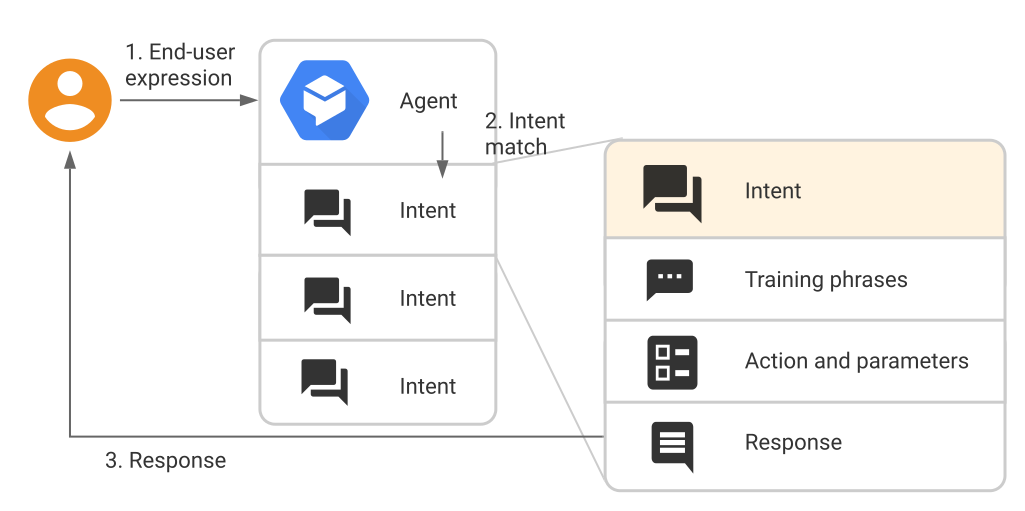
\includegraphics[width=\linewidth]{img/intent-example.png}
\textcolor{myblue}{Entities:} Dienen um einzelne Wörter aus Sätzen auszulesen und zu mappen. Es gibt die Möglichkeit mehrere Trainingsbegriffe zu definieren und auch Synonyme für gleiche Wörter. Auch gibt es die Möglichkeit System-Entities zu verwenden (Vordefinierte Entities, wie Datum und Zeit) \\
\\
\textit{Beispiel: What is the \textcolor{blue}{temperature} going to be \textcolor{orange}{tomorrow} in \textcolor{red}{Seattle}?
Durch das Wort \textcolor{blue}{temperature} versteht der Bot, dass ein Forecast gefragt ist (Intent).}
\\
\textit{Die Wörter \textcolor{orange}{tomorrow} und \textcolor{red}{Seattle} sind Entities für eine Zeit resp einen Ort.}\\
\\
\textcolor{myblue}{Dialog Control (Kontexte):}
Mit Kontexten kann man definieren welcher Intent als nächstes aufgerufen werden sollte, wenn man ein Intent abgeschlossen
hat und kann auch Parameter übergeben, die dann im nächsten Intent verfügbar sind:
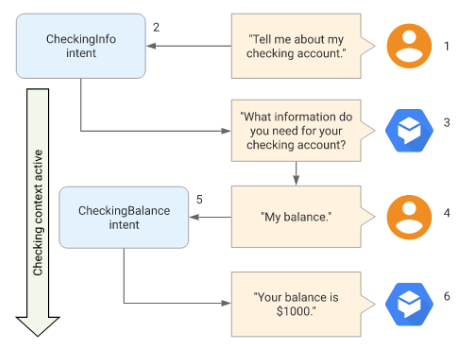
\includegraphics[width=\linewidth]{img/dialog-control.png}
\section{Natural Language Processing (NLP)}
Automatisches erfassen von menschlicher Sprache (gesprochen oder geschrieben). Wichtiger Teilbereich in AI. Ziel ist zu verstehen was ein Mensch will. Kürzlich grössere Fortschritte gemacht. Derzeit ist aber verstehen und auch das Antworten immernoch sehr schwierig für eine KI.\\
Was schon gut funktioniert sind Suchmaschinen, Sprachassistenten(Google Assistant, Alexa) oder Übersetzer (Deepl).
\\
\textcolor{myblue}{Grundlagen Machine-Learning-Projekt:} Die ersten 4 Punkte (Data, Cost-Function, Model, Optimization Procedure) sind die Grundlagen. Die anderen drei benötigt man für verbessertes Machine Learning.
\subsection{Data}
Datenset das gegeben ist inklusive der Pre-Prozess-Pipeline unter anderem mit folgenden Funktionen
\begin{itemize}
\item \textbf{Cleansing}: Aufräumen, Korrigieren und sortieren
\item \textbf{Feature-Engineering}: Extrahieren von Features, z.B Katze ist ein Säugetier (Beziehungen)
\item \textbf{Data-Argumentation}: Daten vervielfältigen durch manipulation (Spiegeln, Farbänderung) oder hinzufügen neuer Date
\end{itemize}

\subsection{Cost-Function (Loss)}
Mathematischer Ausdruck der sagt wie gut oder schlecht Aufgabe gelöst wurde. Dies anhand Angabe einer Zahl. Mean Squared Error (MSE) wird häufig genutzt. Weiter gibt es Domain-Spezifische Kosten.
\\
Beispiel: Gesichtserkennungsalgorithmus. Nun muss man Kosten schätzen wenn Gesichtserkennung falsch positiv oder falsch
negativ ist. Je nach Ort kann es andere Auswirkungen haben. (Access-Control bei CIA oder Identifizierung von Kunden, die viel
Geld ausgeben in einem Geschäft)
\subsection{Model}
Der Teil, der aus einem Input einen Output generiert. Kann einfach sein (Linear $y_i = ax_i + b$) oder komplexes neuronalesNetzwerk mit Millionen von Parameter.
\\
Typischerweise verwendet man Framework wie Tensorflow oder Pytorch
\\
Unterschiedliche Aufgaben benötigen unterschiedliches Modell (Regression, Entscheidungsbaum)
\subsection{Optimization Procedure}
Modell muss nun durch Machine-Learning optimiert werden. Dazu braucht es einen Algorithmus. Optimierungsprozedur nimmt alle oben genannte Elemente und schraubt so lange an Parameter rum, bis das optimale Ergebnis rauskommt.
\\
Beispiele: Stochastic Gradient Descent (SGD), ADAM, RMSProp, ...
\subsection{Performance Optimization}
Bauen von effizienten Pipelines ist schwierig. Deshalb sollten Tool-spezifische Empfehlungen und Referenz-Implementationen zur Hilfe genommen werden.
\subsection{Visualization and evaluation of the Learning Process}
Man kann Lernprozess visualisieren. Man kann also Zeigen ob der Optimierer was sinnvolles tut. Hier kann Tensorboard genutzt werden.
\subsection{Cross-Validation und Regularization}
Ziel ist Modelle zu trainieren, die Gut generalisieren. AI soll eine gewisse Flexibilität haben. \\
Beispiel: Hundebilderkenner soll auch neue Hunderaussen automatisch erkennen.
\subsection{}
Am einfachsten nutzt man dazu Vektoren, welche Wörter auf Grund Ihrer Meinung intepretieren.
\subsection{Vorgehen 1: One-Hot Representation}
Jedem Wort wird ein Vektor zugewiesen mit einem einzigen 1 Wert und alle anderen Werte auf 0 gesetzt.\\
Vektordimeinsion = Anzahl unterschiedliche Wörter
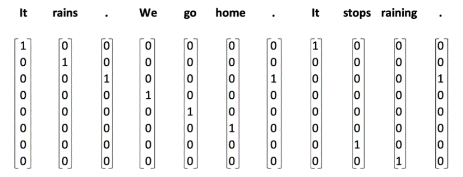
\includegraphics[width=\linewidth]{img/one-hot.png}
Nachteile:
\begin{itemize}
\item \textbf{High dimensional}: Vektoren können schnell sehr grosswerden (Wikipedia-Artikel hat schnell 100'000 Wörter)
\item \textbf{Sparse}: Jeder Vektor hat nur eine 1 und dann viele Nullen. (1 zu 99'999 im Wikipediabeispiel). Sind sehr Memory-Ineffizient und KI kann davon nicht viel lernen
\item \textbf{No generalization}: Es fehlt der Kontext. Alle Wörter sind unabhängig voneinander und es kann keine Bedeutung abgeleitet werden (Z.B Ananas und Birne sind Essen)
\end{itemize}
\subsection{Vorgehen 2: Indexing}
Man macht eine Liste von Wörter und weist diese eine Nummer zu. So benötigt ein Satz nur ein einziger Vektor. Sehr ähnlich wie der One-Hot-Vektor. Aber etwas besser. Deshalb wird Indexing meist als Preprocessing-Step genutzt.
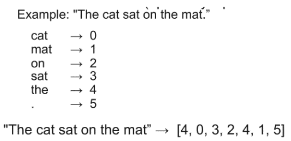
\includegraphics[width=\linewidth]{img/indexing.png}
\subsection{Vorgehen 3: Distributed Representation (dense vectors)}
Ein Wort kann definiert werden mit einem Kontext. Wörter mit ähnlicher Schematik teilen oft den Kontext (cat and rat = Animals)
\\\\
Beispiel: "Look at that little furry mukawibuu with white paws climbing a tree" $\rightarrow$ Mukawibuu wird wohl einem Koala ähneln
\\\\
Bei Distributed Representation wird dieses Konzept genutzt gemacht. Ein Wort, welches indexiert wurde, wird mit einem Algorithmus (Embedding Layer) zu einem Vektor umgewandelt.
\\
\textbf{Word embedding} = Wörter in Vektoren umwandeln, welche die Bedeutung enkodieren.
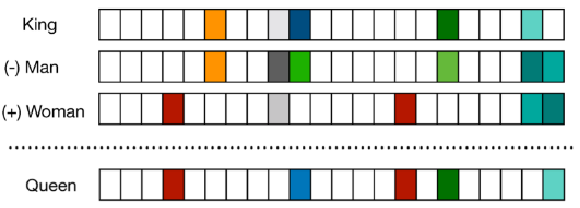
\includegraphics[width=\linewidth]{img/distrubuted-representation.png}
\\
Mit guten Vektoren kann man dann durch Mathematik Ähnlichkeiten erkennen oder durch Addition/Subtraktion neue Wörter bilden. Dazu wird das Skalarprodukt verwendet. Somit kann der Computer mittels Mathematik die Ähnlichkeiten von unterschiedlichen Wörter erkennen.

\begin{itemize}
\item Skalarprodukt zwischen zwei Vektoren ist maximal, wenn beide in die selbe Richtung zeigen
\begin{itemize}
\item Haben beide Vektoren die Norm 1, dann ist das Maximum 1
\end{itemize}
\item Skalarprodukt zwischen zwei Vektoren ist null, wenn die Vektoren senkrecht (orthogonal) zueinander stehen
\item Skalarprodukt zwischen zwei Vektoren ist minimal (negativ), wenn beide Vektoren in entgegengesetzte Richtung zeigen
\begin{itemize}
\item Haben beide Vektoren die Norm 1, dann ist das Minimum -1
\end{itemize}
\end{itemize}

\subsection{Cosine Distance (Kosinusdistanz)}
Das Skalarprodukt wird verwendet für die Cosine-Distance (Kosinusdistanz). Ähnliche Wörter haben eine ähnliche Kosinusdistanz.
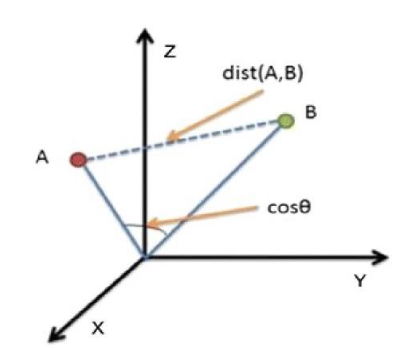
\includegraphics[width=\linewidth]{img/cosine_distance1.png}
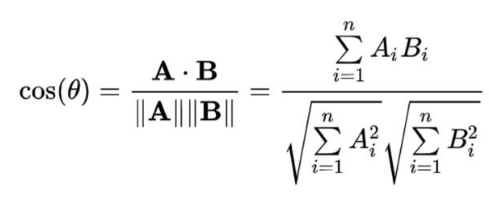
\includegraphics[width=\linewidth]{img/cosine_distance2.png}

\textcolor{myblue}{Skalarprodukt:}\\
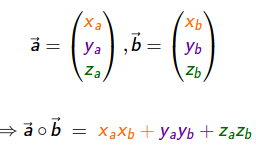
\includegraphics[width=\linewidth]{img/skalarprodukt.png}
$$\frac{dotP\left(e,m\right)}{norm\left(e\right)\cdot norm\left(m\right)}$$
Vektor erstellen = Menu -> 7 -> 1
dotP = Menu -> 7 -> C -> 3\\
norm = Menu -> 7 -> 7 -> 1\\

\subsection{Rechenbeispiel}
Berechne die Kosinusdistanz zwischen Elefant und Maus, sowie zwischen Elefant und Bike.\\
Im Taschenrechner kann folgende Formel gebraucht werden:\\
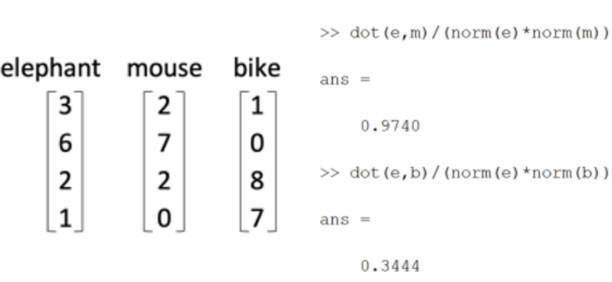
\includegraphics[width=\linewidth]{img/elefant_maus.png}
Elefant und Maus sind sich sehr ähnlich, weshalb die Kosinusdistanz mit 0.974 nahe bei 1 ist. Elefant und Bike ähneln sich nicht.
\section{Introduction to Probability}
\subsection{Zufallsvariable}
Eine Zufallsvariable X (oder anderer Grossbuchstabe) ist eine Variable, die einen numerischen Wert x (Kleinbuchstabe) zuordnet, welche aus einem Zufallsexperiment kommt.\\

Es gibt zwei Arten von Zufallsvariablen:
\begin{itemize}
\item \textbf{Diskret}: X nimmt einen fixen Wert an aus einer fix definierten Zahlenmenge: {1.56, 2.93, 4, 6, 8}
\item \textbf{Stetig}: X nimmt einen Wert aus einem unzählbaren bereich. Z.B alle Zahlen im Intervall (2, 7)
\end{itemize}

Vergleich mit anderen Variablen:
\begin{itemize}
\item \textbf{Algebra}: In einer expression ‘x+2=10’ ist eine variable ein wert, wo eine Gleichung in einen richtigen Ausdruck bringt.
\item \textbf{Programmierung}: Hier ist einer Variable eine Zuweisung. Die Variable kann ihren Wert mit jeder Neuzuweisung ändern.
\end{itemize}
\textbf{Pr(Hurry| spam) = Given that the email is spam, what is the probability that the email contains “Hurry”?
Pr(Hurry| not-spam) = Given that the email is not-spam, what is the probability that the email contains “Hurry”?}
\\\\
Vor der Ausführung eines Zufallsexperiments ist das beste, das wir machen können eine Liste mit allen möglichen Werten mit den zugehörigen Wahrscheinlichkeiten.

Beispiel mit Würfel:

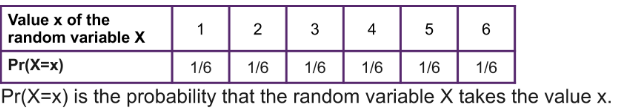
\includegraphics[width=\linewidth]{img/dice.png}

\subsection{Wahrscheinlichkeitsfunktion (Probability Mass Function PMF)}
Die Wahrscheinlichkeitsfunktion einer diskreten Variable ist eine Funktion, welche die Warscheinlichkeit angibt für jeden möglichen x-Wert. Als Beispiel kann man das obige Beispiel mit dem Würfel anschauen. Sie definiert auch eine Wahrscheinlichkeitsverteilung (Probability Distribution). Wird meist als Synonym verwendet.
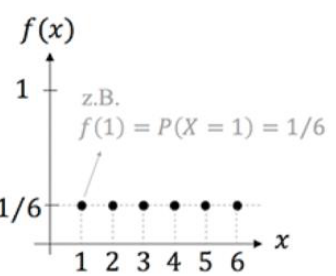
\includegraphics[width=\linewidth]{img/pmf.png}

\subsection{Zwei Zufallsvariablen}
Man kann auch zwei Zufallsvariablen gleichzeitig ansehen. Z.B X ist Augenzahl von Würfel 1 und Y ist Augenzahl von Würfel 2. Dann kann das Zufallsexperiment sein, dass man zwei Würfel wirft, was 36 Möglichkeiten gibt. Jede Möglichkeit ist gleich wahrscheinlich.
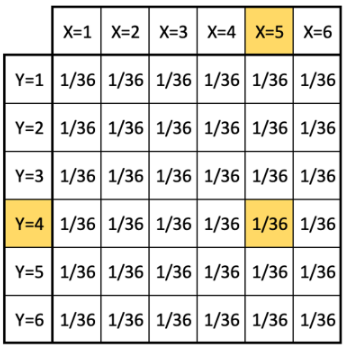
\includegraphics[width=\linewidth]{img/zwei_zufallsvariablen.png}

\subsection{Zusammengesetzte Warscheinlichkeit (Joint Probability Mass Function)}
Die zusammengesetzte Wahrscheinlichkeit oben beschreibt z.B die Warscheinlichkeit das Augenzahl Y=4 und Augenzahl X=5 ist. Diese beträgt 1/36. Man schreibt dies auch Pr(X=5, Y=4) = 1/36 oder P(5,4) =  1/36

\textcolor{myblue}{Unabhängig:}
Im oben genannten Beispiel sind die beiden Zufallsvariablen unabhängig. Ein Würfelwurf beinflusst das andere Exgebnis nicht. Also gilt folgende Formel:\\
P(X, Y) = P(X) * P(Y)     (wenn X und Y unabhängig sind)\\
P(X, Y, Z) = P(X) * P(Y) * P(Z)    (wenn X, Y und Z unabhängig sind)

\textcolor{myblue}{Bedingte Warscheinlichkeit (Correlated Random Variable):}
Doch unabhängig ist eher die Ausnahme als die Regel. Meist sind die Variablen Abhängig voneinander. \\
Joint Probability P(X,Y) und Conditional Probability P(X|Y) (X wenn Y) sind wie folgt miteinander verknüpft:\\
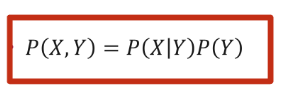
\includegraphics[width=\linewidth]{img/correlated_random_variable.png}
Aus der Joint Probability kann man auf die Marginal Probability schliessen aber nicht umgekehrt, da die Marginal Probability eine Summe ist.
\textcolor{myblue}{Satz von Bayes:}\\
Ebenso gilt der Satz von Bayes:\\
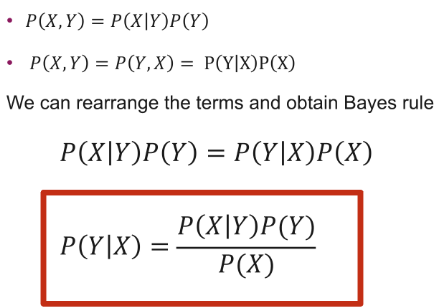
\includegraphics[width=\linewidth]{img/bayes.png}
TODO include examples
\input{content/woche04}
\section{Datenvisualisierung}
Datenvisualisierung bedeutet Daten grafisch darzustellen. Dies ist ein erster Schritt in Machine Learning.\\
Visualisierung von Daten hilft um...
\begin{itemize}
\item ... ein intuitives Verständnis der Daten zu erhalten
\item ... Trends, clusters und lokale Muster zu sehen und identifizieren, welche man bei Raw-Daten sehr schwer sieht
\item ... Entdecken von Ausreissern und ungewöhnliche Gruppen
\item ...Trends zu identifizieren, cluster zu sehen
\item ..unsere Hypothesen/Vermutungen/Theorien zu validieren
\item ... Resultate von Umfragen, etc. zu visualisieren. (Dies sollte man bei wichtigen Nachrichten tun, da Leute meist nur die
\item Grafiken in einem Report ansehen, wenn sie diesen überfliegen.)
\end{itemize}
Datenvisualisierungen können auch überraschende Fakten aufdecken.
\subsection{Plots}
Mithilfe der Python Bibliotheken Mathplotlib und Seaborn (moderner, nutzerfreundlicher) können Daten visualisiert werden.
Um Daten zu importieren ist Pandas eine sehr hilfreiche Phyton-Bibliothek.\\
Ein Plot benötigt dringend nachfolgende Informationen:
\begin{itemize}
\item Label der X-Achse: Was für Daten werden in der X-Achse präsentiert?
\item Label der Y-Achse: Was für Daten werden in der Y-Achse präsentiert?
\item Titel: Was zeigt der Plot
\item Skala: Es muss entschieden werden zwischen Linear und Logarithmisch. Je nach dem andere Aussagekraft und besser geeignet. Beispiel Daten Moores Law: Transitoren pro Mikroprozessor. Hier ist logarithmisch besser geeignet, da es da es den Trend der Verdoppelung besser zeigt. Linear sieht so aus als wäre lange nichts passiert.
\item Dimension der Daten: 2D oder 3D ist das einzige was dargestellt werden kann und der Mensch auffassen kann. Mehr Dimensionen wie Wörtervektoren können nicht dargestellt werden oder müssen heruntergebrochen werden auf wenige Dimensionen
\end{itemize}

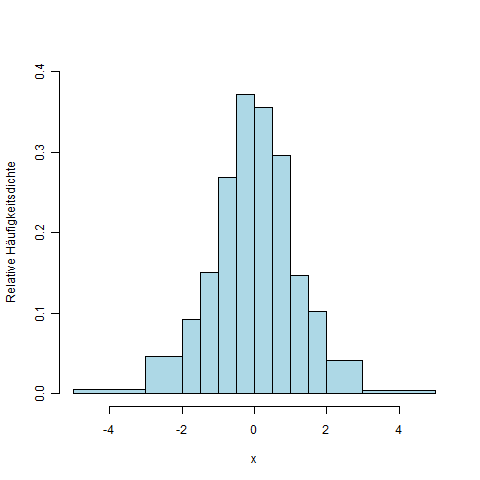
\includegraphics[width=\linewidth]{img/histogram.png}
Balken = Bins\\
\textcolor{myblue}{Box Plots und Violin Plots:}\\
Anzeigen von Daten anhand der Aufteilung in Quartile und Median. Zeigt sehr gut Aussreiser an und wo sich die meisten Daten befinden.
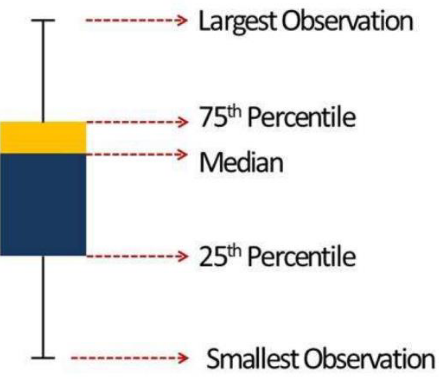
\includegraphics[width=0.9\linewidth]{img/boxplot.png}
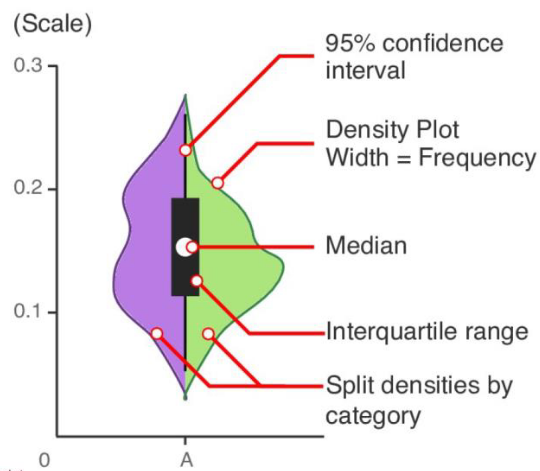
\includegraphics[width=0.9\linewidth]{img/violinplot.png}
\textcolor{myblue}{Streudiagramm (Scatter Plot)}\\
Zum Verständnis der Beziehung zwischen zwei kontinuierlichen Variablen kann ein Streudiagramm verwendet werden. Dabei kann eine Farbe verwendet werden um eine dritte Variable zu kodieren. Hilft dabei, eine Vorstellung vom Grad der Korrelation einer Variablen mit der anderen zu erhalten.
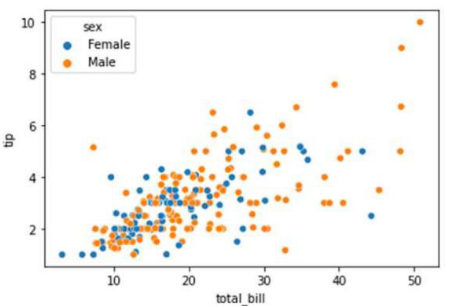
\includegraphics[width=\linewidth]{img/scatterplot.png}
\textcolor{myblue}{Auswahl Plot}\\
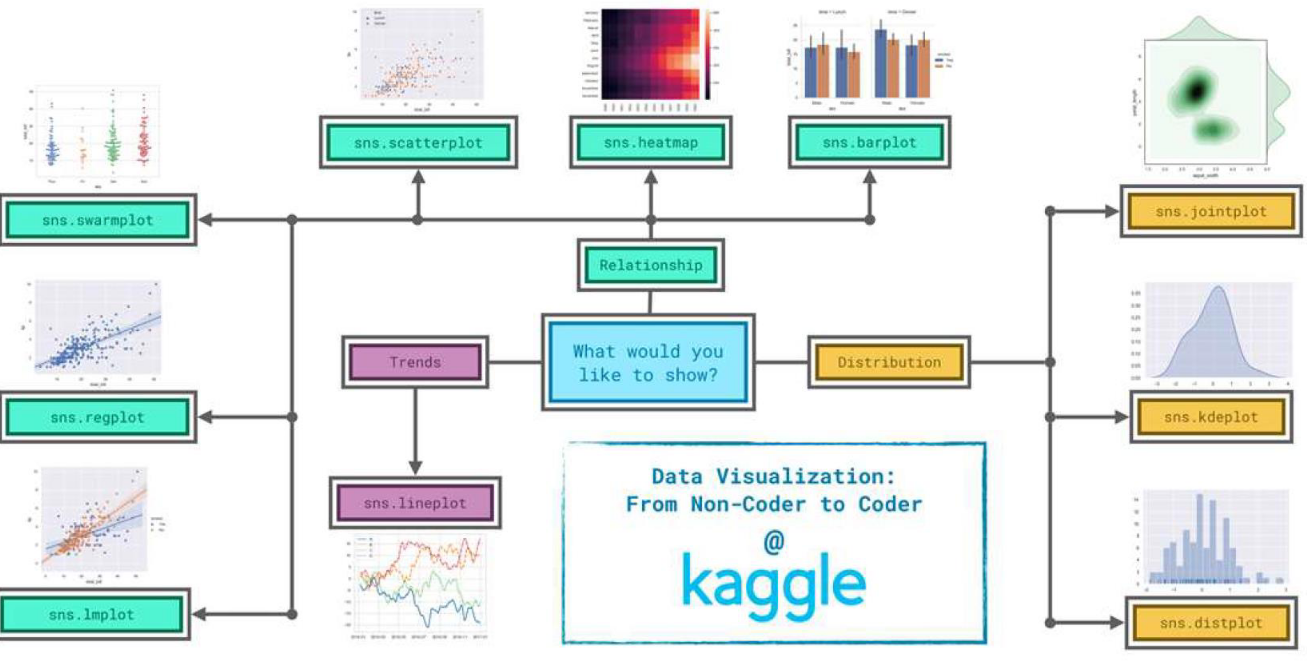
\includegraphics[width=\linewidth]{img/which_plot.png}
\section{Lineare Regression}
Lineare Regression ist eine einfache Methode um Daten zu analysieren.\\
Man nutzt es hauptsächlich für:
\begin{itemize}
\item \textbf{Interpretation}: Verstehen ob ein bestimmter Input ein Effekt hatfür den Output. Bsp: Gibt es eine Beziehung zwischen Raucher undLungenkrebs?
\item \textbf{Prediction}: Voraussehen wann was in Zukunft passieren könnte.Z.B. Wann geht eine Maschine kaputt anhand von Sensoren für Öldruck und Temperaturen
\end{itemize}
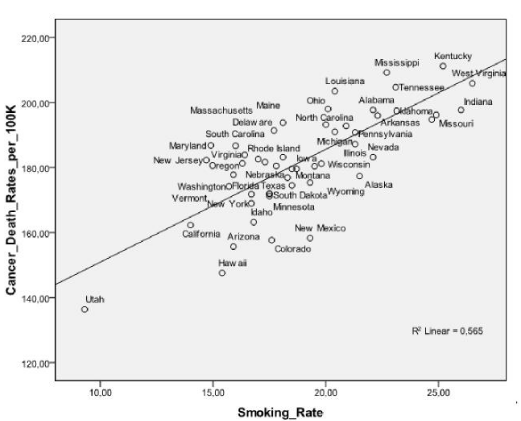
\includegraphics[width=\linewidth]{img/linear_regression.png}
\subsection{Linear Regression und Machine Learning}
Lineare Regression wird von Statistik «ausgeliehen». Hier ist es ein Beispiel von Algorithmen oder Techniken aus dem supervised learning. Wir haben also Inputdaten X und die Labels (In unserem Fall Y). Dann wird ein einfacher Algorithmus verwendet um daraus den Linearen Zusammenhang zu sehen. Das Modell soll also lernen Y vorauszusagen.\\
\textcolor{myblue}{Model}\\
In ML Model steht für irgendeine mathematische Funktion, welche die Daten erklärt.
$$y_i \approx f(x_i)$$
$$y_i = f(x_i) + \epsilon_i$$

Das $\epsilon_i$ steht für «unerklärtes Rauschen». Man nimmt an, dass die der normalen Distribution folgt.\\
Die Funktion f kann beliebig kompliziert sein (Konstante oder Multi-Millionen-Parameter-Netzwerk). Machine Learning muss das korrekte Modell finden, welche die Daten möglichst gut interpretiert. Anstelle die Funktion näherungsweise zu bestimmen, bestimmen wir ein y-Hut, welche eine Schätzfunktion von $y_i$ ist.
$$y^\wedge_{i} = f(x_i)$$
In der Linearen Regression wird nur die Lineare Represäntation angeschaut zwischen input und output. Vor dem Lernen vom Algorithmus bestimmen wir den Model-Space (Funktionenschar). In einfachsten Fall sind x und y skalar und wir haben nur zwei frei wählbare, unbekannte Variablen a und b. Diese müssen wir nun mit Machine Learning bestimmen um möglichst nah an den Daten zu sein.
$$y^\wedge_{i} = a * x_i + b$$
a wird meist \textbf{slope} genannt und b \textbf{intercept}.\\
\textcolor{myblue}{Mean squared Error MSE (Loss, Residuals)}\\
Dies ist das \textbf{Loss} das wir minimieren wollen. (Hinweis: MSE ist normalerweise mit 2 dividiert)
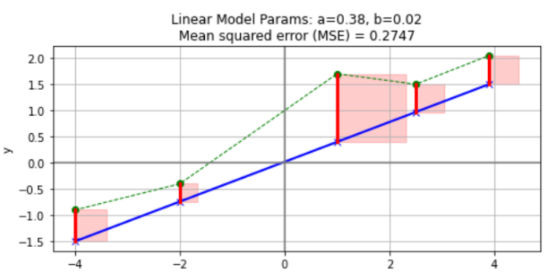
\includegraphics[width=\linewidth]{img/mse.png}
$$y^\wedge_{i} = a * x_i + b$$
$$e_i=y_i-y^\wedge_{i}$$
$$E=\frac{1}{2N}\sum_{i=1}^N e^2_i$$
$$=\frac{1}{2N}\sum_{i=1}^N(y_i-(a * x_i + b))^2$$
\subsection{Korrelation und Kausalität}
Korrelation ist \textbf{nicht} Kausalität!\\
Auch wenn der Koeffizient 0 ist können die Daten strukuriert sein -> Keine Aussagen über Kausalität machen. Immer Daten visualisieren und ebenso die Residuals.
\subsection{Komplexere Lineare Modelle}
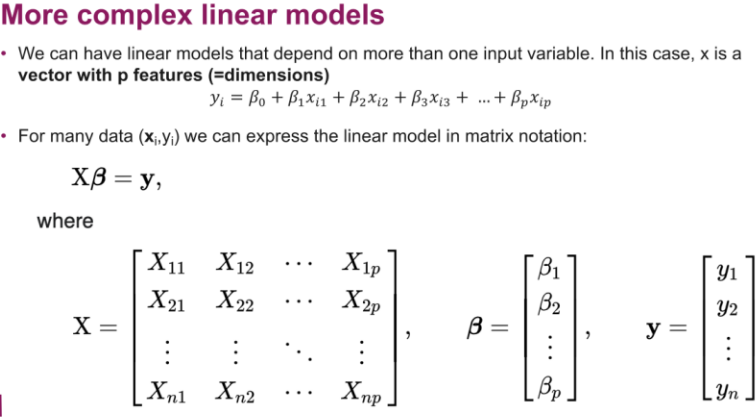
\includegraphics[width=\linewidth]{img/komplexere_lineare_modelle.png}
\subsection{Uniform Distrubution, Normal Distribution}
Die Gleichverteilung (Uniform Distrubution) beschreibt eine Zufallsvariable, die jeden Wert innerhalb eines bestimmten
Intervalls annehmen kann. Jeder Wert in diesem Intervall ist gleich wahrscheinlich.\\
Bei der Normalverteilung (Gausian Distrubition) ist die Zufallsvariable an der Normalverteilung angelehnt.\\
rng.normal(loc=0, scale=1, size=10000)\\
loc=Mittel, Scale=Standardabweichung, size=Anzahl Samples
$$x = Sollmenge (Sollfüllmenge)$$
$$ \mu = Momentaner Wert (Füllmenge)$$
$$ \delta = Standardabweichung $$
Stlg -> Menu -> 5 -> 8\\
( A, B ) == [Sollfüllmenge, Sollfüllmenge]
\subsection{Seaborn Jointplot}
Der Jointplot ist eine Verbindung von zwei Variablen mit bivariaten und univariaten Graphen. Es zeigt die (empirischen) Randverteilungen als Histogramme. Das Ergebnis ist ideal: die Daten (x-Werte) sind gleichmäßig über den gesamten Bereich verteilt (Gleichverteilung in -50/+50), während die Residuen bei 0 zentriert sind (Standardnormalverteilung).
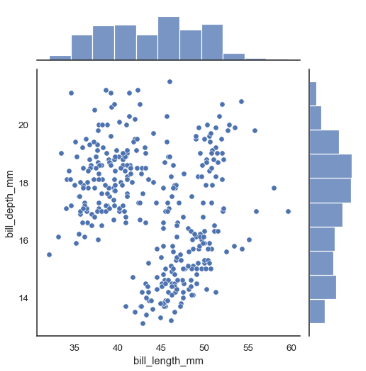
\includegraphics[width=0.9\linewidth]{img/seaborn_jointplot.png}
\section{Grundbegriffe}
\subsection{7 Steps of Machine Learning}
\begin{enumerate}
\item Gathering Data: Daten Sammeln, die fürs Training und Evaluieren genutzt werden können
\item Data Preparation: Daten randomizen und zusammenstellen. Ebenso visualisieren um zu schauen ob komplett genug.Weiter müssen Daten gesplittet werden in Training Data und Evaluation Data (80\%/20\% oder 70\%/30\%). Somit kannman mit Daten Testen, welche nicht Im Training vorhanden waren
\item Choosing a model: Ein Modell auswählen das passt (Musik, Text, Zahlen, Linear)
\item Training: Mit den Trainingsdaten das Modell trainieren. Dabei immer wiederholen bis zufrieden
	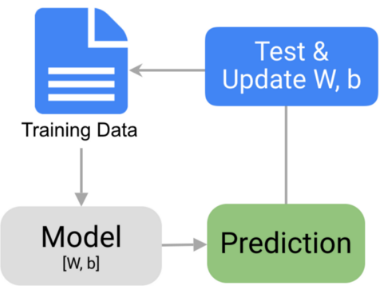
\includegraphics[width=\linewidth]{img/machine_learning_training.png}
\item Evaluation: Mit Evaluationsdaten testen ob Training gut genug.
\item Parameter Tuning: Experimentieren mit weitern Parameter um Training zu verbessern. «Hyperparameter»
\item Prediction: Model nutzen um nun mit anderen Daten eine Aussage machen zu können (Modell anwenden)
\end{enumerate}

\subsection{Bias and Variance}
\textcolor{myblue}{Bias}\\
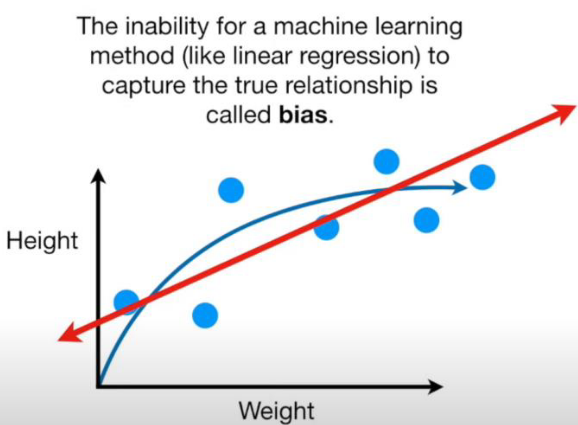
\includegraphics[width=\linewidth]{img/bias.png}
Da die gerade Linie nicht wie die \textit{wahre} Beziehung gekrümmt werden kann, weist sie einen relativ grossen Bias auf.
\textcolor{myblue}{Variance}
Differenz der Nähe der Daten (Sum of Squares) zwischen Test und Evaluationsdaten wird Varianz genannt.
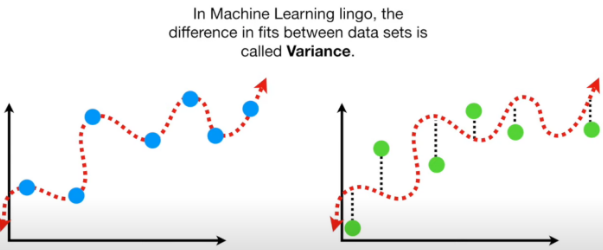
\includegraphics[width=\linewidth]{img/variance.png}
\subsection{Optimization: Stochastic Gradient Descent (SGD)}
Eine alternative \textbf{Optimierungsfunktion} SGD.\\
\textbf{Error-Function der linearen Gleichung:}
$$E = \frac{1}{2N} \sum_{i=1}^N e^2_i =\frac{1}{2N} \sum_{i=1}^N (y_i - (a*x_i+b))^2$$
\begin{itemize}
\item \textbf{Gradient} (in Vektor Ableitung nach \textbf{a} und einmal nach \textbf{b} und dies in einem Vektor platzieren
    $$ Gradient \: of \: E =$$
    $$\begin{bmatrix}
       \frac{\delta E}{\nabla a} \\
       \frac{\delta E}{\nabla b} \\
     \end{bmatrix}
         = 
    \begin{bmatrix}
    \frac{1}{N} \sum_{i=1}^N (y_i - (a * x_i + b))(-x_i) \\
       \frac{\delta E}{\nabla b}(y_i - (a * x_i + b))(-1) \\
     \end{bmatrix}
    $$
\end{itemize}
Problem hier: Der normale Gradient dient dazu von einem Tal auf einen Berg zu kommen, also vom Minimum zum Maximum, zudem macht er noch zu grosse Schritte (Bild 1). Dies läsen wir indem wir noch ein alpha hinzufügen und die Werte negieren (Bild 2):
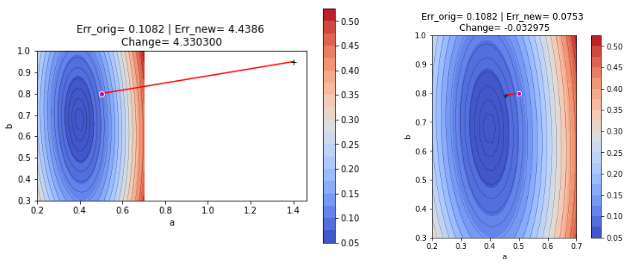
\includegraphics[width=\linewidth]{img/gradient_schritt.png}
Um nun weiterzukommen und immer näher ins Tal zu kommen zum minimalen Error, müssen wir nun am neuen Punkt wieder den Gradient berechnen:
\\
    $\begin{bmatrix}
       a \\
       b \\
    \end{bmatrix}_{t+1}
     = 
    \begin{bmatrix}
       a \\
       b \\
    \end{bmatrix}_{t}
     - \alpha     
    \begin{bmatrix}
       \frac{\delta E}{\nabla a} \\
       \frac{\delta E}{\nabla b} \\
    \end{bmatrix}
    |_{
    \begin{bmatrix}
       a \\
       b \\
    \end{bmatrix}_t
    }
    $
\\
Dies geht so lange weiter bis man eine bestimmte Anzahl Iterationen erreicht hat, die vorgegeben wird. Daraus ergibt sich eine Learning-Kurve. In diesem Beispiel ist schon nach 20 iterationen das Ziel beinahe erreicht und nur noch am b wird optimiert.
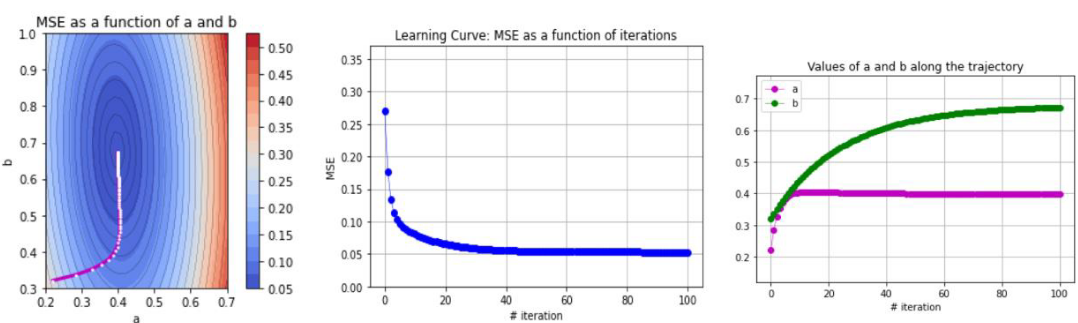
\includegraphics[width=\linewidth]{img/gradient_learning_curve.png}
\textit{Hinweis: Hat man mehr als ein Tal, dann muss man einfach an mehreren Punkten starten und so versuchen das Globale Minimum zu finden (Mehrere Punkte unterschiedliches Minimum, dann den tiefsten nehmen)}\\\
\textbf{Hier noch ein Bild, welches die Idee noch veranschaulicht:}\\
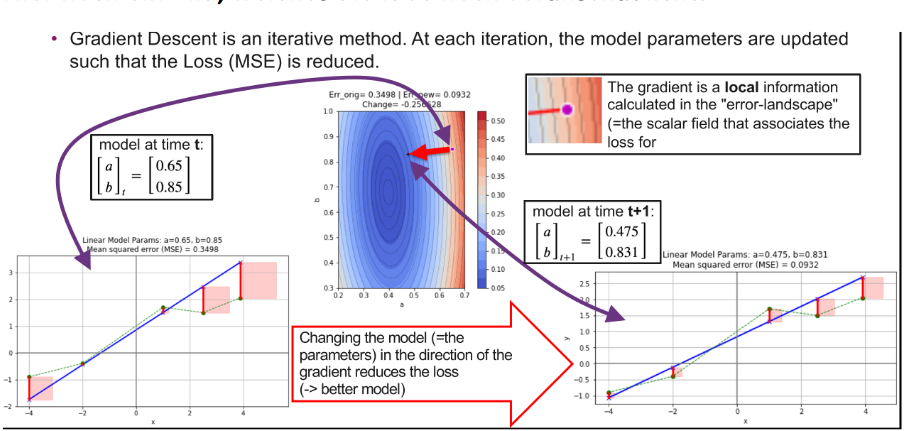
\includegraphics[height=0.7\linewidth, angle=90]{img/gradient_explanation.png}
\subsection{Stochastic Gradient Descent (SGD)}
SGD hilft das (lokale) Minimum zu finden. Man startet random an verschiedenen Punkten, damit die Chance das globale Minimum zu finden grösser ist. In jedem Schritt wird der\textbf{ ganze Parametervektor} optimiert.
Hier ist das Ziel, dass man nur eine kleine Menge and Datenpunkte nimmt um die Fehler und so den Gradient zu berechnen. Man selektiert also random ein paar Datenpunkte aus dem Dataset (J = Teildatenset):
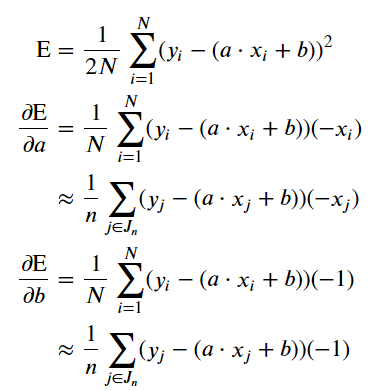
\includegraphics[width=0.7\linewidth]{img/sgd_formula.png}\\
Dies führt zur folgender Update-Regel mit welcher man den Parametervektor berechnen kann (bei uns musste nie abgeleitet werden und das Ableitungszeichen konnte ignoriert werden):
    $$\begin{bmatrix}
       a \\
       b \\
    \end{bmatrix}_{t+1}
     = 
    \begin{bmatrix}
       a \\
       b \\
    \end{bmatrix}_{t}
     - \alpha     
    \begin{bmatrix}
       \frac{\delta E}{\nabla a} \\
       \frac{\delta E}{\nabla b} \\
    \end{bmatrix}
    |_{
    \begin{bmatrix}
       a \\
       b \\
    \end{bmatrix}_t
    }
    $$
Nun versucht man den Batch auf 1 zu wählen oder möglichst klein (32 oder 64 werden häufig verwendet).\\
\textit{Hinweis: Bei Batch 1 kann es sehr grosse Zicksacke geben, da ja für einen Punkt mehr als eine Lösung gibt und MSE auch 0 sein kann. Dennoch kommt man irgendwann auf eine Lösung, doch es gibt Zickzackwerte bei der Lerning-Kurve. Und nahe beim Ziel geht er wieder weiter weg. Dieses Problem kann aber auch gelöst werden indem man Alpha immer kleiner wählt.}
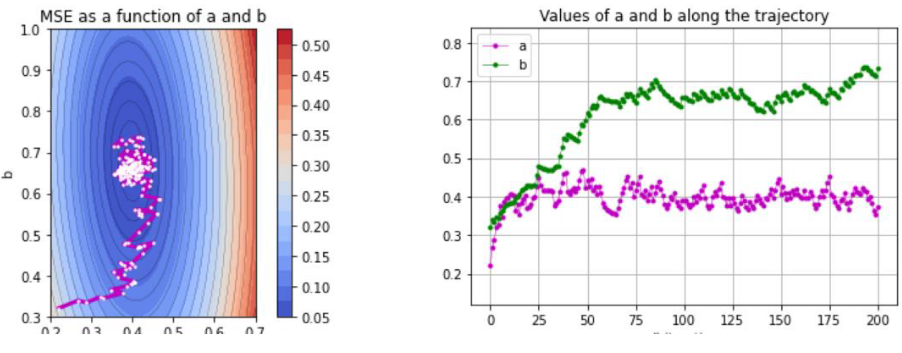
\includegraphics[width=\linewidth]{img/sgd_learning_curve.png}
\subsection{Stochastic Gradient Descent with annealed learning rate}
Wie oben erwähnt gibt es eine grosse Streuung am Ende und man erreicht nicht mehr so genaue Werte. Dem kann man entgegenwirken indem man immer alle paar Iterationen alpha(Lernrate) verkleinert. Somit flacht es nach ein paar Iterationen immer mehr aus und man kommt anfangs sehr schnell in die Mitte:
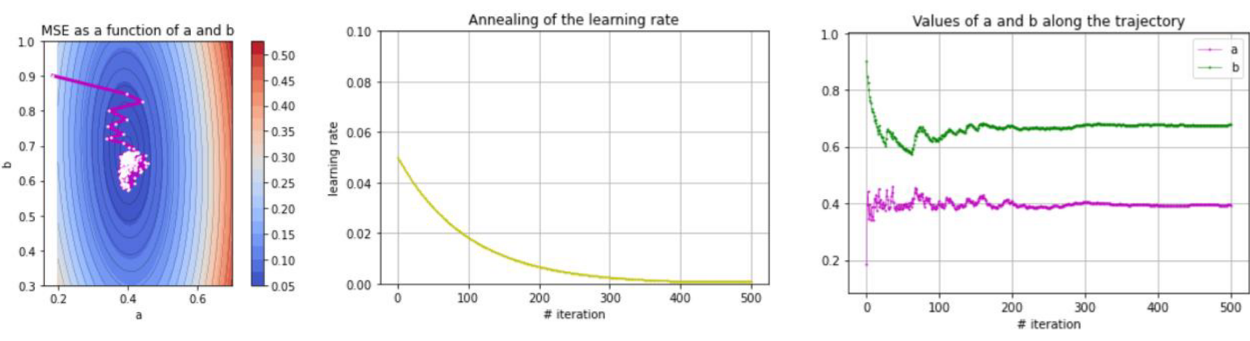
\includegraphics[width=\linewidth]{img/sgd_annealed_learning_curve.png}

\subsection{Allgemeine Anmerkungen}
\begin{itemize}
\item Diese Methode geht nur, wenn die Loss-Function ableitbar ist.
\item SGD kann nur mit einem Datenset arbeiten, was sehr ineffizient ist und selten benutzt wird
\begin{itemize}
\item Batch oder Minibatch-Gradient ist also besser
\end{itemize}
\item SGD muss der Gradient berechnen. Ist dies schwer?
\begin{itemize}
\item Ja, wenn man es selbst tun muss und es viele Parameter gibt. (Neurale Netze können Millionen Parameter haben)
\item Nein, wenn man ein Modell hat und ein Machine Learning Framework nutzt (Tensorflow, Pytorch).
\end{itemize}
\item Gradient Descent ist ein Basis Baustein für viele weitere Algorithmen wie Adam, Adagrad, RMSProp, etc.
\end{itemize}

\section{Generalisation und Regularisierung}
\subsection{Overfitting}
Overfitting ist wenn alle Punkte genau getroffen werden. Dann stimmt es zwar für die Trainingsdaten genau, aber sobald weiter Datenpunkte dazukommen stimmt es für diese nicht mehr. Wir haben zwar einen MSE von 0, dies ist aber ein \textbf{In-Sample Error (Training Error)}. Der Loss wurde sehr stark minifiziert in der Trainingsphase.\\
\\
Sobald wir dann aber die Testdaten dazu nehmen (Neue noch nicht gesehene Daten, haben wir dann einen grossen \textbf{Out Of
Sample Error (Generalization Error)}. Ein gutes Modell hat ein tiefen Generalization Error.\\
\\
Ziel: tieferer Generalization Error, In-Sample Error darf aber grösser sein
\subsection{Underfitting}
Underfitting tritt dann auf, wenn das Modell zu einfach ist. Wir haben ein viel zu hoher In Sample Error, als auch ein zu grosser Generalization Error. Ein Beispiel dafür wäre eine Gerade, welche durch ein sehr komplexes Model durchgeht und sehr viel verpasst. Gegenteil von Overfitting.
\subsection{Generalization Error}
Der Generalization Error kann nicht berechnet werden, sondern nur geschätzt werden. Wir müssen mit den Daten arbeiten, die wir haben. Deshalb müssen wir unsere Daten splitten in Test- und Trainingsdaten. Ein guter Split ist 80\% Training und 20\% Test. So nutzt man die Training-Daten um das Modell zu trainieren und wenden dann mit den Testdaten das Modell an. Der Test-Fehler ist eine Schätzung vom Generalization Fehler.
\subsection{Bias und Varianz}
Wenn wir die beiden Fehler genauer mathematisch analysieren können wir zwei Werte feststellen: Bias und Varianz.\\
\textcolor{myblue}{High Bias, Low Variance}\\
In diesem Fall ist das Modell zu einfach. Egal wie viele Daten wir haben, das Modell gibt keine besseren Ergebnisse. Zum Beispiel wir nehmen ein Lineares Modell obwohl es passendere gibt. Dann ist dieses zu einschränkend. Die rote Linie wird bei vielen Daten gleich bleiben auch wenn ich ein neuer Punkt hinzufüge. Wir haben underfitting.\\
\textcolor{myblue}{Low Bias, High Variance}\\
Man nimmt ein (zu) komplexes Modell. Es kann die Daten besser beschreiben. Beispiel 6 Punkte und wir nehmen ein Polynom Grad 5. Hier passt das Modell genau zu den Testdaten. Aber wir haben nun Overfitting.Die Varianz ist hoch. Ein weiter Datenpunkt führt dann zu einem sehr grossen Generalization error. Und sobald ein Punkt etwas verschoben ist, ist die Line komplett eine andere.
\subsection{Regularisierung}
Unser Ziel: Wir wollen möglichst eine tiefe Varianz. Der Bias ist eher sekundär, sollte aber auch möglichst tief sein. Man braucht aber die optimale Balance. Am besten schauen wir da den Training- und Testerror genauer an. Es gibt einen Punkt wo der Testerror am tiefsten ist und dann wieder steigt je genauer das Modell ist. Dazu verwenden wir Regularisierung.
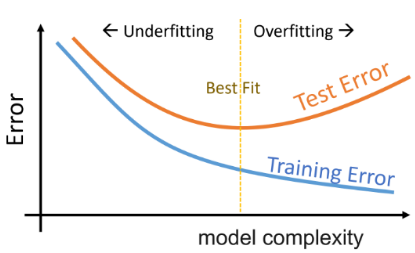
\includegraphics[width=\linewidth]{img/regularization.png}
Regularisierung fügt Constrains hinzu, ein Penalty-Term (Cost-Function). Der Optimizer optimiert die Daten (MSE minimalisieren) sowie auch den Constraint.
Es gibt zwei Zutaten die wir benötigen:
\begin{enumerate}
\item Weg zum Modell-Komplexität zu messen
\begin{itemize}
\item L1 Norm (Lasso) 
$$\sum_{j=1}^p | \beta_j|$$
\item L2 Norm (Ridge)
$$\sum_{j=1}^p \beta^2_j$$
\end{itemize}
\item Weg zum Model-Komplexität zu kontrollieren
\begin{itemize}
\item Penalty-Term wird zu Loss hinzugefügt
\item Komplexere Modelle haben höhere Penalty
\item Constraint wird zum Optimierungsprozess hinzugefügt
$$\sum_{i=1}^n(y_i-\sum_{j=1}^p x_{ij} \beta_j)^2+ \lambda \sum_{j=1}^p \beta^2_j$$
\end{itemize}
\end{enumerate}

«Lamda ist der Hyperparameter»\\
Lamda = 0: dann haben wir kein Constraint also nur MSE. Vergrössern von Lamda: zu grosse Bias, kleinere Varianz\\
\textbf{Beispiel}: Wenn man zwei Modelle gegeben hat, die mit verschiedenen Regulasierungswerten($\lambda$) trainiert wurden, dann wähle das Modell, das im Schnitt die besseren Werte erzielt. Bei grösseren Regulasierungswerten ($\lambda$) erhält man tiefere Varianz, aber höheres Bias. Doch bei einer grossen Varianz soll man ein neues Modell trainieren, mit dem Besseren Regularisierungswert($\lambda$).
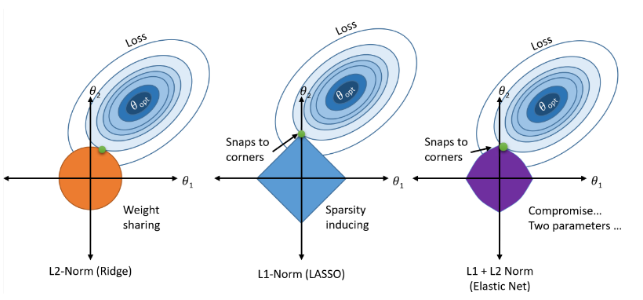
\includegraphics[width=\linewidth]{img/l-norm.png}
\section{Cross-Validation}
Ohne Cross-Validation: Test-Fehler basiert auf 20\% der Daten.\\
Funktionsweise der k-Fold-Crossvalidation: Daten werden zuerst geshuffelt. Anschliessend aufgeteilt in k-Fold (Üblich: 5-Fold, 10-Fold. Gibt aber auch N-Fold wo jeder Fold nur ein Datenpunkt hat). Dann wird jedes mal ein anderer Fold als Test-Datensatz genommen und das Modell trainiert.\\
\textit{Hinweis: Daten in einem Fold ändern sich während den einzelnen Splits nicht. Diese bleiben über die ganzen Trainings gleich. Weiter muss die Preprocessing-Pipeline während den einzelnen Splits laufen und nicht davor, da sonst Ergebnisse verzerrt werden.}
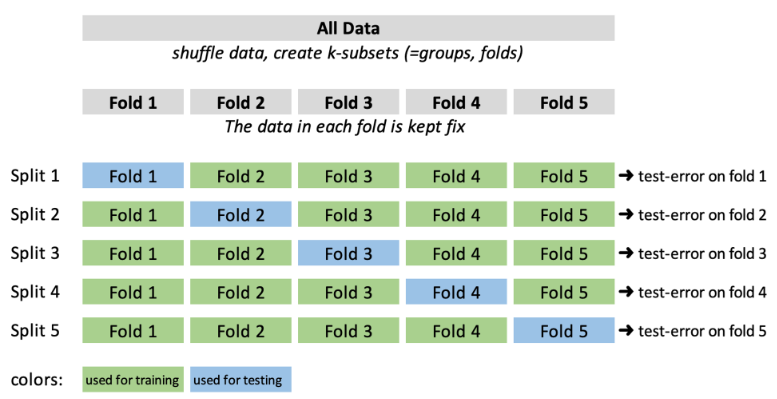
\includegraphics[width=\linewidth]{img/cross-validation.png}
\subsection{Ziel 1: Generalisierungsfehler schätzen}
Hier wird aus den einzelnen Testfehler der Durchschnitt genommen und so der Mean und die Variance des Testfehlers genommen. Ist genauer als mit einzelnen Tests.
\subsection{Ziel 2: Auswahl von Hyperparameter}
Man variert mit den Hyper[arameter (Regularisierungslamda, etc.) und findet so den optimalen Parameter $\lambda_{opt}$ heraus
\subsection{Scikit-learn Cross-Validation}
Einzelne Daten werden vorher ganz rausgenommen als Testdaten. Dann wird mit anderen Cross-Validation gemacht. Wird meist empfohlen.
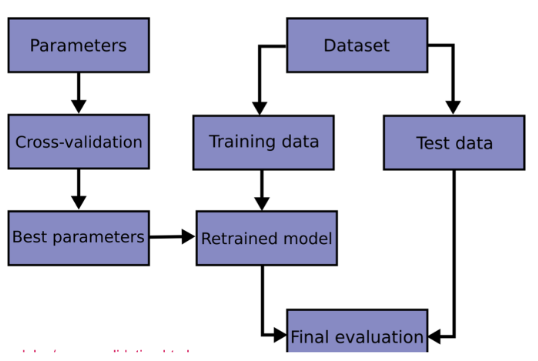
\includegraphics[width=\linewidth]{img/scikit-cross-validation.png}
\section{Artificial Neural Networks}
AI ist inspiriert von unserem Gehirn und den Neuronen. Die biologischen Neuronen wurden vereinfacht in ein Artificial Neuron. Diese bieten ein Input-Vektor. Jedes Neuron hat seine eigenen Input-Gewichte und ein Bias (Intercept). Sie berechnen die Summe von den gewichtenten Inputs (Skalarkprodukt), fügen Bias hinzu und passen es in eine nichtlineare Aktivierungsfunktion. Nachfolgend ein Beispiel eines einfachen Netzes:
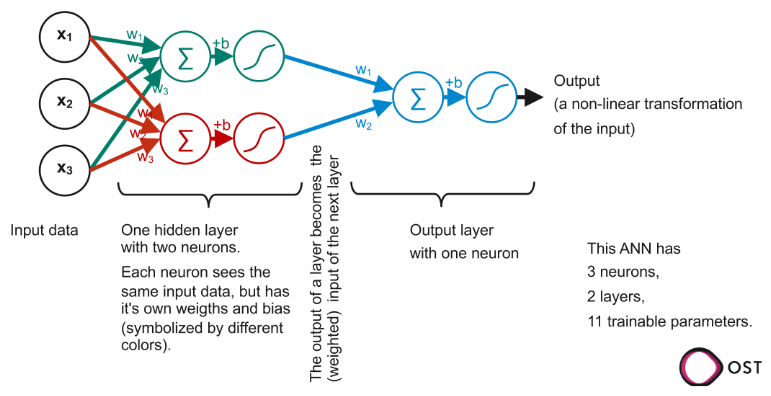
\includegraphics[width=\linewidth]{img/neural-network.png}
Hat ein Netz zahlreiche Hidden Layer, dann wird von einem \textbf{Deep Neural Network} gesprochen.\\
\\
Ein ANN ist eine Datenstruktur zur Definition beliebig komplexer mathematischer Funktionen.
\begin{itemize}
\item ANNs sind aus (vielen) relativ einfachen Ausdrücken zusammengesetzt.
\item Ein ANN ist ein Ausdrucksbaum. Jeder Knoten kann ausgewertet werden.
\end{itemize}

\subsection{ANN trainieren}
\begin{itemize}
\item Wir betrachten einen einfachen Fall von \textbf{supervised learning}: Für jede Eingabe $\vec{x}_i$ erhalten wir die Ausgabe $y_i$ (bekannte Ausgaben werden gewöhnlich als \textbf{Zielwerte} oder \textbf{Labels} bezeichnet)
\item Das ANN wird mit zufälligen Gewichten initialisiert und erzeugt eine Ausgabe $\hat y$. Dann wird ein Optimierer (z. B. SGD) eine Kostenfunktion (z. B. MSE).
\item Das heißt, bei jeder Iteration und für jedes einzelne Gewicht w(und jeden Bias b) wird die partielle Ableitung $\frac{\delta}{\delta w}(y- \hat y)^2$ berechnet werden muss. Glücklicherweise gibt es einen Algorithmus, der dies sehr effizient macht: \textbf{Backpropagation}.
\end{itemize}

\section{Logistic Regression}
Hier geht es um Daten die Binär klassifiziert werden (Ja-Nein Fragen). Beispiel: Wird es Hageln aufgrund eines Satellitenbilds. Oder hat jemand bald ein Epsilepsie-Anfall wegen einem EEG reading. \\
\\
In solchen Fällen sehen die Daten anderst aus, weshalb wir ein anderes Modell und Loss-Funktion brauchen. (Lineare Funktion geht nicht) Für den Optimizer können wir aber weiterhin Gradient Descent verwenden, da die andere Loss-Funktion convex ist.
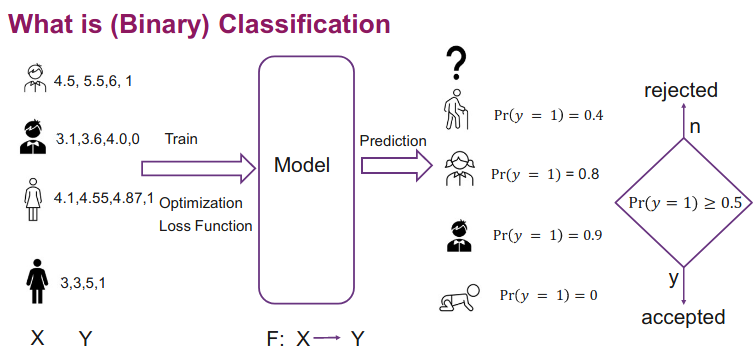
\includegraphics[width=\linewidth]{img/binary_classification.png}
\subsection{Warum nicht Lineares Modell?}
Das Problem der Linearen Regression ist, dass die Kurve ganz anders aussieht, sobald ein weiterer Datensatz dazu kommt und Tresholding hier falsche Ergebnisse liefern kann. Die Kostenfunktion (Loss) Min Squared Error funktioniert hier gar nicht und liefert diese falschen, verzerrten Ergebnisse. Wir sind aber interessiert in eine Warscheinlichkeits-Output. Somit brauchen wir ein Modell, dass die Wahrscheinlichkeit abbildet.
\subsection{Sigmoid Funktion}
Die Lösung ist die Sigmoid-Funktion. Sie bietet genau das benötigte Modell:
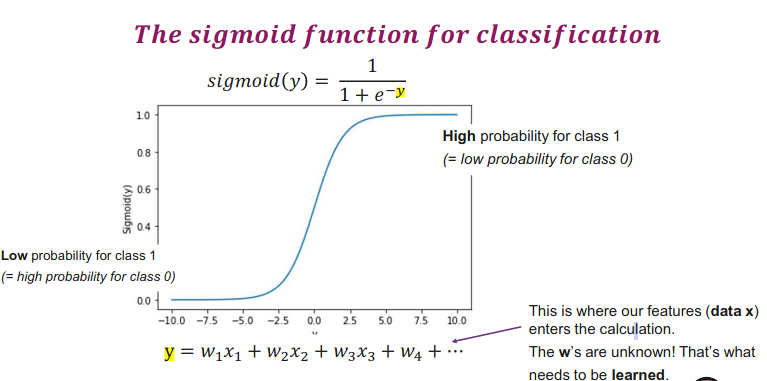
\includegraphics[width=\linewidth]{img/sigmoid.png}
Das y bzw. manchmal auch z kann alle Dimensionen enthalten. z.B.
$$y = w_1x_1=w_2x_2+w_3x_3+...$$
\subsection{Wahrscheinlichkeit}
Wir können die geschätze Wahrscheinlichkeit so schreiben:
$$Pr(y=1|x;W) = Pr(y=1 | x) = p(x) = \frac{1}{1+e^{-(W^Tx)}}$$
Für eine Vorhersage können wir schreiben $ p(x) = \frac{1}{1+e^{-(W^Tx)}}$ wobei man beachten sollte, dass p eine Zahl zwischen 0 und 1 ist.\\
\textbf{Wir haben nun das Modell aber wie bekommen wir W?}
\subsection{Maximum Likelyhood (Loss)}
Wenn man alle Datenpunkte (X, Y) hat, wollen wir die Wahrscheinlichkeit maximieren, dass alle Vorhersagen richtig sind (oder die Wahrscheinlichkeit minimieren, dass alle Vorhersagen falsch sind)!
Das Ziel des Trainings ist die Festlegung der Koeffizienten W so einzustellen, dass p nahe bei 1 liegt, wenn y = 1 und W nahe bei 0 liegt, wenn y = 0
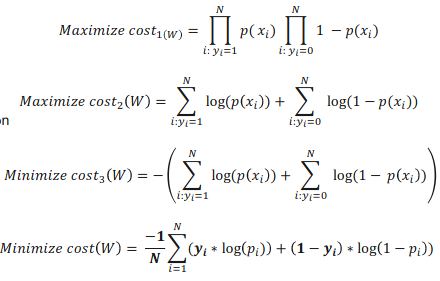
\includegraphics[width=\linewidth]{img/maximum_likelyhood.png}
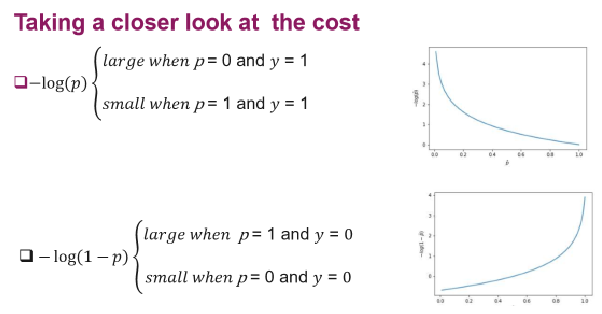
\includegraphics[width=\linewidth]{img/maximum_likelyhood_cost.png}
\section{Classifier Evaluation}
Wir stellen uns die Frage ob das Model gut genug ist, weshalb wir das Modell genauer evaluieren. Dazu nutzen wir unter anderem eine Confusion Matrix.
\subsection{Confusion Matrix}
\textbf{False Positive:} Der berechnete Wert ist 1 und der wahre Wert ist 0. (Fälschlicherweise richtig)\\
\textbf{False Negative:} Der berechnete Wert ist 0 und der wahre Wert ist 1. (Fälschlicherweise falsch)\\
\textbf{True Negative:} Der berechnete Wert ist 0 und der wahre Wert ebenso. (Korrekt)\\
\textbf{True Positive:} Der berechnete Wert ist 1 und der wahre Wert ebenso. (Korrekt)\\
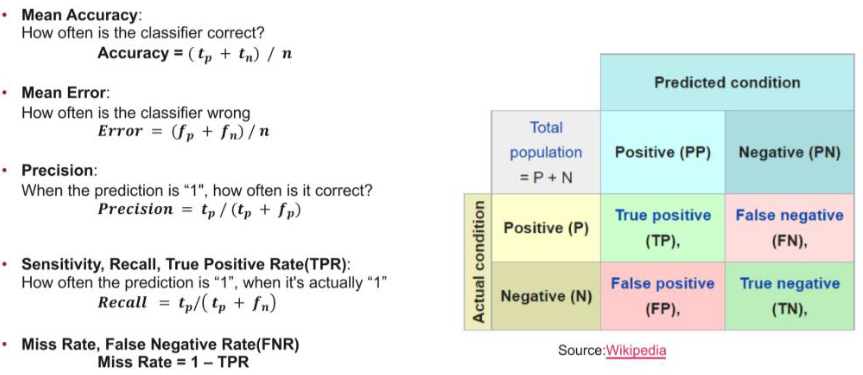
\includegraphics[width=0.8\linewidth]{img/confusion_matrix.png}
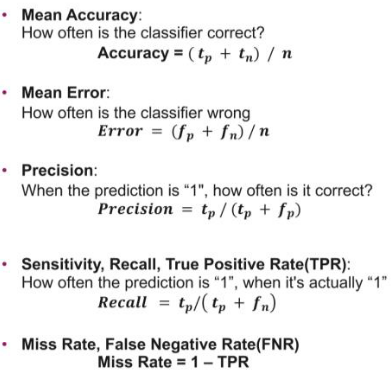
\includegraphics[width=0.8\linewidth]{img/confusion_matrix_description.png}
Bei oben genannten Formeln ist die Mean Accuracy nicht genug um bestimmen zu können, ob wir ein gutes Modell haben. Beispiel: Dataset wo 90\% Nein und 10\% Ja sind. Das Modell sagt nun einfach immer Nein. Hier ist dann die Accurracy bei 90\%. Nun schauen wir die weiteren Werte an Precision und Recall. Diese sind in diesem Modell jeweils 0...
\subsection{Precision vs Recall}
Es kommt drauf an worauf man den Fokus legt je nach Applikation. Nachfolgend die Folie dazu:
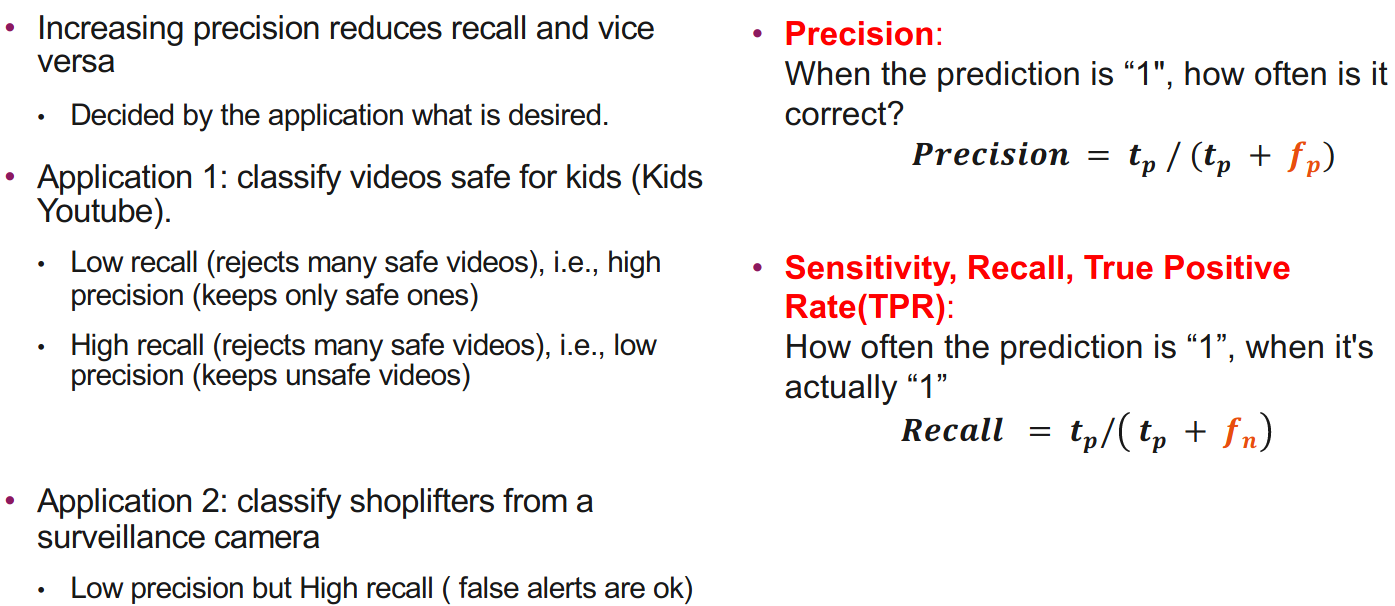
\includegraphics[width=\linewidth]{img/precision_vs_recall.png}
\subsection{Threshold}
Was der Threshold angeht gibt es keine allgemeingültige Lösung mittels Mathematik. Hier kommt es wieder auf die Applikation drauf an. (Threshold ab wann True/False). Vorgehen um das Threshold zu bestimmen:
\begin{enumerate}
\item Modell trainieren
\item Predictions machen mit dem Test-Set
\item Versuchen unterschiedliche Threshold-Werte zu verwenden und damit folgendes berechnen:
\begin{itemize}
\item True Positive Rate (Wie oft richtig akzeptiert) $TPR = t_p/(t_p + f_n)$
\item False Positive Rate (Wie oft falsch akzeptiert) $FPR = f_p/(f_p + t_n)$
\end{itemize}
\item Wir erhalten unterschiedliche TPR und FPR Werte. Diese können wir Plotten -> Ergibt ROC Space (Anderer Plot mit Precision und Recall könnte ein Schnittpunkt ergeben, was sicher ein sehr guter Punkt ist)
\end{enumerate}
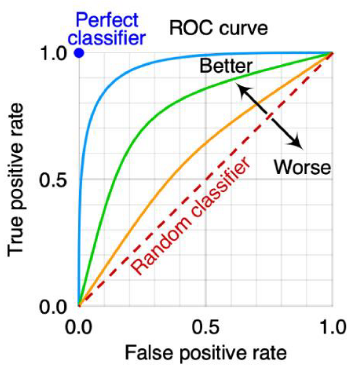
\includegraphics[width=0.6\linewidth]{img/treshold.png}\\
Eine ROC-Kurve ist ein grafisches Diagramm, das die Diagnosefähigkeit eines binären Klassifizierungssystems veranschaulicht, während seine Unterscheidungsschwelle variiert wird. \\
Die ROC-Kurve wird erstellt, indem die Rate der echten positiven Ergebnisse (TPR) gegen die Rate der falschen positiven Ergebnisse (FPR) bei verschiedenen Schwellenwerten aufgetragen wird.
\section{K-Nearest-Neighbours (KNN)}
Haben wir Plots, welche mehr als zwei Klassen haben brauchen wir eine weiter Variante und Logistic Regression wird hier nicht funktionieren. Weiter wird ein lineares Modell nicht zufriedenstellende Ergebnisse Liefern und nicht überall funktionieren:
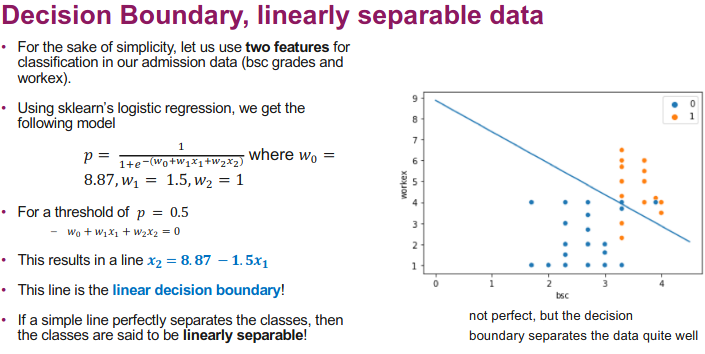
\includegraphics[width=\linewidth]{img/decision_boundary.png}
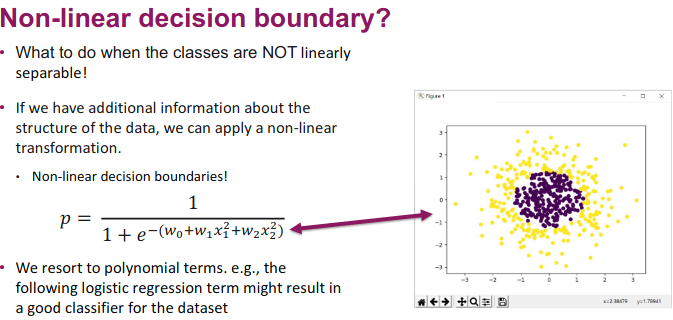
\includegraphics[width=\linewidth]{img/non_linear_decision_boundary.png}
Beispiele für Plots mit mehr als 2 Klassen: SARS-CoV-2 Varianten (Alpha, Beta, Gamma, etc.), Wetter (Sonnig, Wolkig, Regen, Schnee)\\
Logistic Regression kann hier funktionieren, ist aber sehr umständlich. Mann muss viel trainieren (rekursiv), was langsam ist. So braucht es eine Methode ohne training, mit Predictions, einfacher Support mehrere Klassen, und auch möglichkiet Nicht- Lineare-Modelle zu trainieren. Hier kommt KKN ins Spiel.
\subsection{Funktionsweise}
\begin{enumerate}
\item Training und Testdaten laden
\item Value von k bestimmen (Nummer von Nachbaren, welche berücksichtigt werden sollten (1, 5, 10, 15, ...))
\item Für jeden Test-Datenpunkt
\begin{itemize}
\item Für alle Trainingsdaten muss Distanz berechnet werden d(xtest, xtrain): Mit Euclidean, Manhattan, cosine, ...
\item Trainingdaten müssen in ascending Order sortiert werden
\item Die ersten k Datenpunkte werden von der Sortierung genommen
\item Von diesen Punkte werden die am häufigsten vorkommende Klasse genommen als Klassifikation
\end{itemize}
\end{enumerate}
Key-Elemente: Die Anzahl Nachbarn k, Distanz-Metrik\\
\textbf{Beispiel}: Wenn man einen Punkt einer Klasse zuordnen muss und nichts gegeben ist, dann Manhattan Distanz nehmen und um den Punkt ein Quadrat zeichnen, dass  die nächsten N=12 Nachbarn einschliesst und schauen, von welcher Klasse am meisten vorhanden sind.
\subsection{Distanz-Metriken}
Es gibt unterschiedliche Definitionen von Distanzen, die verwendet werden können.
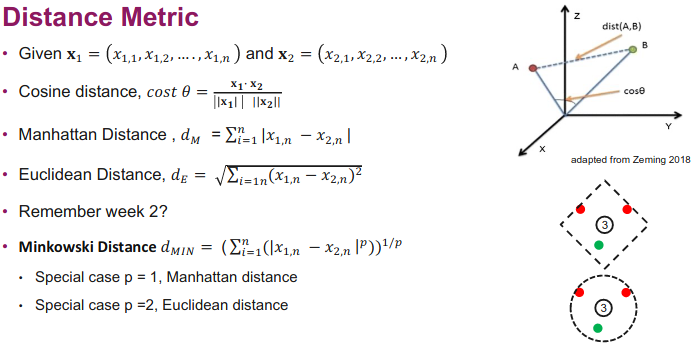
\includegraphics[width=\linewidth]{img/distance_metric.png}
\subsection{Das richtige k und die richtige Distanzmetrik}
Um dies zu bestimmen sollte man folgende Elemente von AI verwenden (Beschrieben in vorangehenden Kapitel):
\begin{itemize}
\item Test-Train split
\item Cross Validation
\item Test Performanceüberwachung (Mean accurarcy, Precision, Recall)
\end{itemize}
\subsection{Vor/Nachteile}
\textcolor{green}{Vorteile:}\\
\begin{itemize}
\item Einfaches Modell
\item Wenige Hyperparameter
\end{itemize}

\textcolor{red}{Nachteile:}
\begin{itemize}
\item K muss gut gewählt werden
\item Grosse Berechnungsaufwand, wenn Sample gross ist
\item Nicht effizient bei vielen Dimensionen
\item Richtige Skalierung muss verfügbar sein
\end{itemize}

\subsection{Beispiel IRIS}
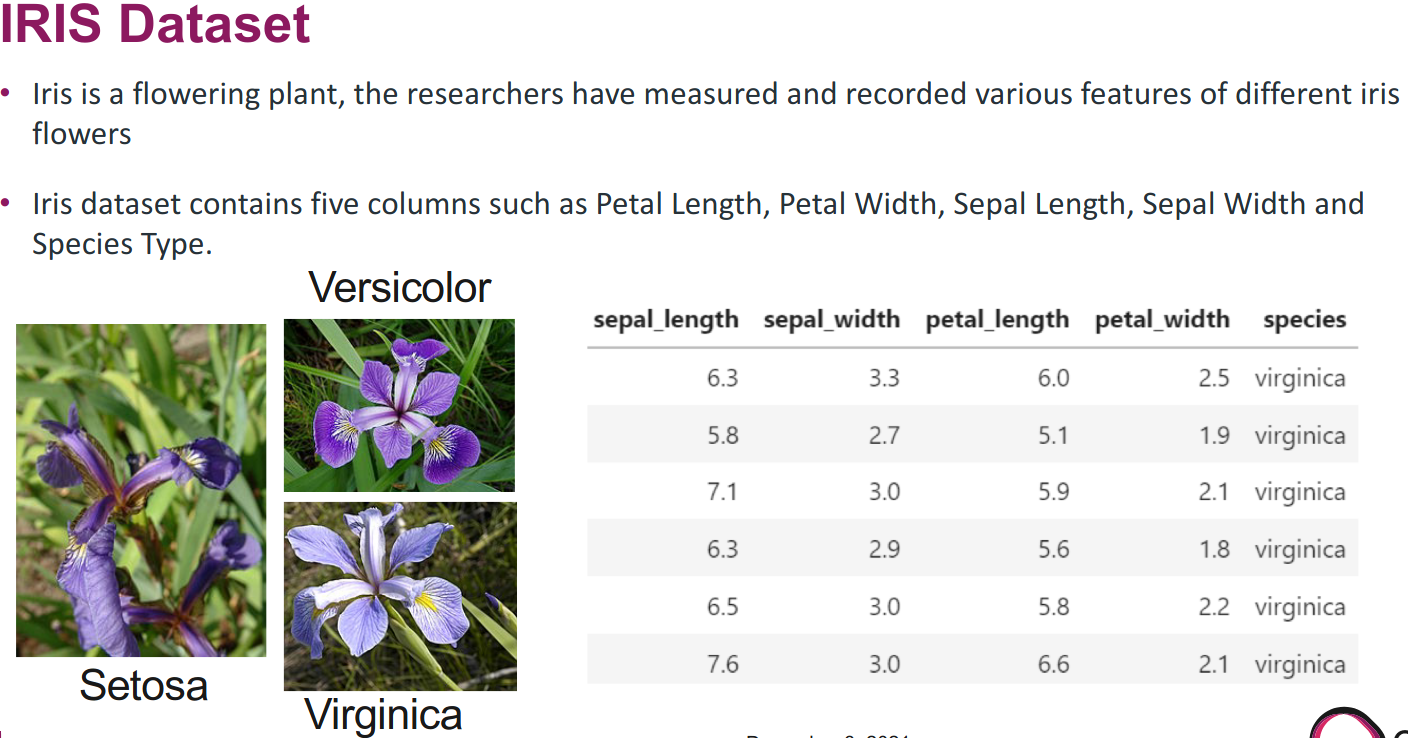
\includegraphics[width=\linewidth]{img/iris.png}
\section{Clustering}
\subsection{Unsupervised Learning}
Alles bisher war Supervised Learning. Nun ist das Thema Unsupervised Learning. Hier haben wir nur die Features (X-Werte) und uns sind die Labels (Y-Werte) unbekannt.\\
Damit können wir die Struktur der Daten lernen. Wir wollen das Pattern der Daten selbst entdecken. Die Struktur kann auch durch Noise Verborgen sein. Menschen können Struktur sehr leicht erkennen und Alogrithmen haben es schwerer. Wo uns aber Algorithmen unterstützten ist bei grossen Daten mit vielen Dimensionen. Wir können maximal 3 Dimensionen haben.
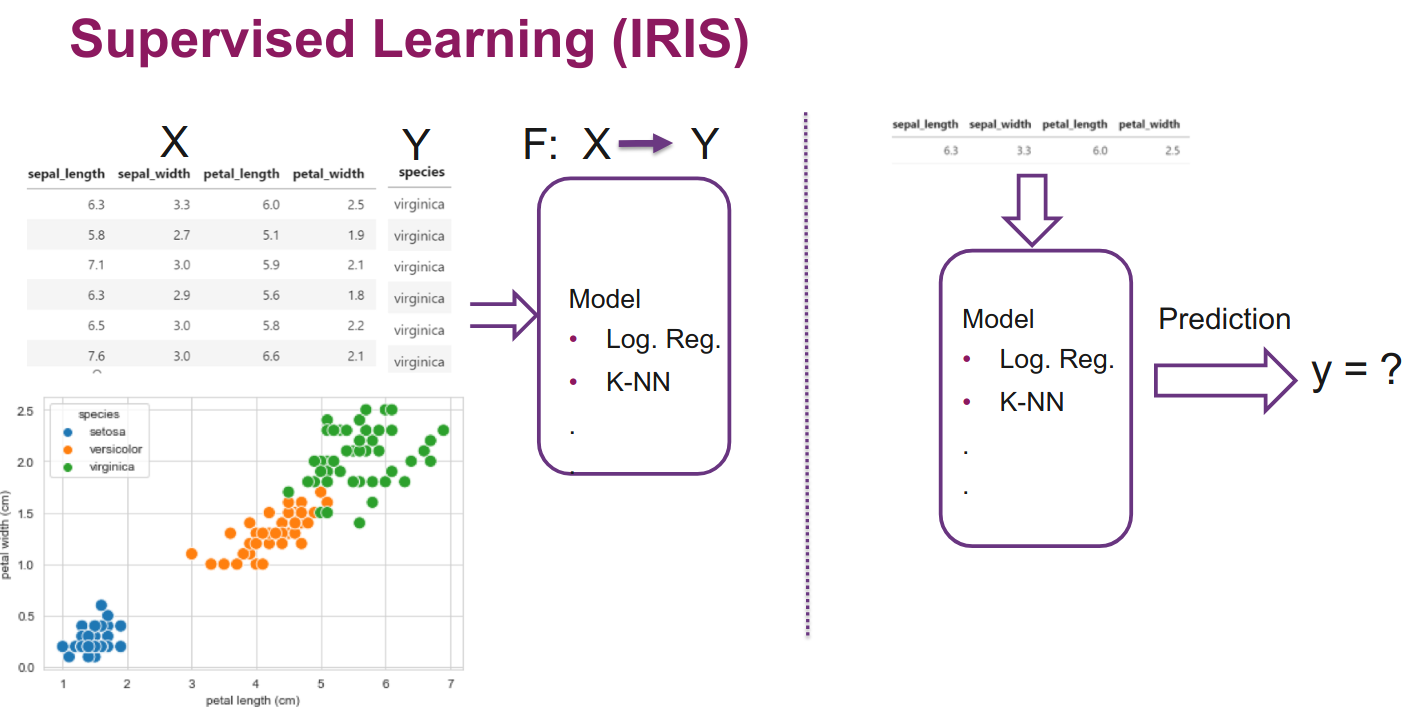
\includegraphics[width=\linewidth]{img/supervised_iris.png}
\includegraphics[width=\linewidth]{img/unsupervised_iris.png}
\subsection{Clustering (Mit KNN Klassifizierung)}
Ein Beispiel, was wir erkennen können mit unsupervised Learning sind Clusters: Datenpunkte mit ähnlichen Werten fallen in einer Gruppe zusammen.\\
\textcolor{myblue}{Beispiele:}
\begin{itemize}
\item Soziale Netzwerke analysieren
\item Astromische Daten
\item Google News (Gruppieren von News in Kategorien)
\item Market Segmentation
\end{itemize}

Wir können KNN Klassifierung zur Hilfe nehmen. Denn wir nehmen an, dass ähnliche Datenpunkte nahe zusammen sind. (Distanzmetriken: Eculidean, Manhatten)\\
\\
Group \textbf{n} data points into $k_c$ number of clusters.
\section{Naive K-means}
Ein Algorithmus um Cluster zu erkennen.
\includegraphics[width=\linewidth]{img/clustering_naive_k-means.png}
\includegraphics[width=\linewidth]{img/k-means_math.png}
\subsection{Stopping-Kriterium}
\begin{itemize}
\item Wenn «Centres» nicht mehr ändern (Zeitaufwändig)
\item Datenpunkte in einem Cluster ändern sich nicht mehr (Geht viel zu lange)
\item Distanz vom Datenpunkt zum Zentrum >= gewählten Threshold
\item Fixe Anzahl an Iterationen erreicht
\begin{itemize}
\item Zu wenig Iterationen: Schlechte Cluster -> Muss gut gewählt werden
\end{itemize}
\end{itemize}
\subsection{Intialisierung}
Die Anfangs-Zentrumswerte sind meist zufällig. Somit ist die Performance davon abhängig. Bestimmte Anfangswerte führen auch zu schlechten Convergence-Raten oder auch schlechtes Clustering. Wenn die Zentrumswerte nahe beieinander sind braucht es viel mehr Iterationen. Am besten also mehrmals ausführen und wenn Cluster stabil bleibt dann haben wir gutes Cluster.
\subsection{Standardisierung}
Die Daten müssen normalisiert werden. Ist wichtig, dass Features mit grossen Werte nicht dominieren.\\
Beispiel: Noten und Berufserfahrung. Ohne Normalisierung hat die Berufserfahrung ein Übergewicht und die Noten spielen keine Rolle.
\subsection{Qualität des Clusters: WCSS und Silhouette}
Die Nummer des Cluster ist ein Hyperparameter, der intelligent gewählt werden muss. Was man bereits im voraus sagen kann. $K_c = 1$ bringt uns nicht weiter (Alle Punkte gehören zum selben Cluster). $K_c = N$ ist viel zu gross, dann haben wir minimalen Abstand zum Zentrum, aber jeder Punkt ist ein eigenes Cluster. Bei Unsupervised Learning haben wir keine Testdaten die wir prüfen können, da wir keine Labels haben zum gegenchecken.
Somit benötigen wir andere Methoden.
\subsection{Within-Cluster Sum-of-Squares WCSS}
Distanz von den Punkten zum Zentrum muss minimalisiert werden.
\includegraphics[width=\linewidth]{img/wcss.png}
\subsection{Silhouette Score}
Entfernung der Punkte von einem Cluster zum anderen Cluster. Desto näher bei 1, desto besser.
Silhoutte Score von einem Punkt $= \frac{b-a}{max(a,b}$\\
a=der durchschnittliche Abstand zwischen den einzelnen Punkten innerhalb eines Clusters.\\
b=der durchschnittliche Abstand zwischen einem Cluster und seinem nächsten Nachbarcluster
TODO: Unterstand Silhoutte Score Pictures in W13
\subsection{Bestimmung welche Clustergrösse anhand von IRIS}
In diesem Beispiel ist die optionale Clustergrösse 2-3 Cluster. Denn ab drei Cluster gibt’s beim WCSS einen Knick und es verbessert sich nicht mehr so stark. Silhouette fällt aber noch weiter.

\section{Ensemble Methods}
Ziel: Mehrere Modelle zu nutzen um ein Problem zu lösen. Anstelle das perfekte Modell zu nutzen, werden mehrere (schlechtere) Modelle trainiert und die Ergebnisse aggregiert.\\
\textbf{Wisdom of Crowd}: Bei einer komplexen Frage mehrere zufällig ausgewählte Personen fragen und Ergebnisse aggregieren. Dies funktioniert wahrscheinlich sehr gut und ist auch einfacher als die am besten passende Person, den Experten zu finden. Dieses Konzept kann mit Ensemble auf Machine Learning übertragen werden. Wir erhalten je nach dem sogar ein viel besseres Resultat als mit nur einem Modell. Ensemble steht für «A group of Predictors», «Ensemble Learning», «Ensemble Method» Ensemble Methoden werden meist gegen ende eines Projekt benötigt, wenn man bereits einige gute Predictors hat und diese kombinieren will.
\subsection{Unterschiedliche Dimensionen}
\textcolor{myblue}{Unterschiedliche Algorithmen}\\
Wir kennen beispielsweise zwei Methoden für die Klassifizierung. Diese können wir kombinieren. Z.B. KNN und Logistic Regression.
\includegraphics[width=\linewidth]{img/diverse_predictors.png}
\textcolor{myblue}{Unterschiedliche Hyperparameter}\\
Wir können bei KNN verschiedene k verwenden. Oder bei Logistic Regression diverse Regularisierungsparameter.\\
\textcolor{myblue}{Unterschiedliche Trainingsdaten}\\
Wir können Cross Validation Nutzen und dann die Ergebnissie kombinieren oder diverse Features aus Feature Engineering kombinieren. So haben wir unterschiedliche Splits.
\includegraphics[width=\linewidth]{img/diverse_training_data.png}
\subsection{Voting}
\textcolor{myblue}{Hard}\\
Beim harten Voting wird die Klasse genommen mit den meisten Votes. Beispiel in der Grafik oben wird Setosa genommen, da
dies zwei mal vorkommt und Versicolor nur einmal.\\
\textcolor{myblue}{Soft}\\
Kann nur genommen werden, wenn Ergebnisse Warscheinlichkeiten sind, nicht Klassen. Dann kann man einen Durschnitt aus
allen Modellen nehmen.
\subsection{Auswählen der Daten (Bagging)}
Für die verschiedenen Modelle müssen die Daten aufgesplittet werden. Da gibt es grob zwei Varianten:\\
\textbf{Sampling without Replacement:} Datenpunkt kann nur einmal selektiert werden. -> Pasting
\textbf{Sampling with Replacement:} Datenpunkt kann mehrmals selektiert werden. -> Bagging (Bootstrap Aggregating)
\includegraphics[width=\linewidth]{img/choose_data.png}
\includegraphics[width=\linewidth]{img/ensemble_method_bagging.png}
Bagging kann auch für Features gemacht werden nicht nur für die Daten. So kriegt man noch mehr unterschiedliche Modelle. (max\_features und bootstrap\_features).\\
Sampling both features and training data -> Random Patches\\
Sampling only features -> Random Subspace\\
\subsection{Out of Bag (oob) Evaluation}
Es gibt Datenpunkte die nie gewählt werden wenn man die Datenpunkte zufällig wählt. Dies sind dann oob-Punkte. Diese können genutzt werden als Testdaten um das Modell zu trainieren. So braucht man nicht extra vorher die Daten aufzuteilen in Trainings- und Testdaten.
\subsection{No free lunch theorem}
Warum Ensemble statt alle Zeit investieren in die Optimierung eines einzelnen Modells? Antwort: Weil kein einzelner Algorithmus die Lösung ist für ein Problem und es keinen besten Algorithmus gibt. Wichtige Punkte die zu beachten sind:
\begin{itemize}
\item Kein einzelner Algorithmus kann alle Probleme besser lösen als jeder anderer Algorithmus
\item Machine Learning muss richtig verstanden werden, genauso die involvierten Daten, bevor man den Algorithmus wählt
\item Jedes Modell ist nur so gut, wie die Daten die wir haben und den Schlüssen, die man daraus zieht.
\item Einfachere Modelle, wie Logistic Regression, tendieren eher dazu zu underfitten und haben mehr Bias. Zu komplexe Modelle führen zu grösseren Varianzen und tendieren zum Overfitting.
\item Die besten Modelle sind jeweils in der Mitte von zwei Bias-Varianzen-Extremen
\item Um ein gutes Modell zu finden, muss man mehrere unterschiedliche Modelle probieren und vergleichen mittels Cross-Validation.
\end{itemize}
\includegraphics[width=\linewidth]{img/bagging_overview.png}


% \newpage
% \section{Logik}
\textcolor{myblue}{Nulläre Funktion:} Funktion mit null Parametern\\
Bsp.: $f() = 1$ \quad		=> eine Möglichkeit mit null Argumenten\\
\textcolor{myblue}{Unäre Funktion:} Funktion mit einem Parameter\\
Bsp.: $f(x) --> x$ \quad	=> Zwei mögliche Argumente: x=0 oder x=1\\
\textcolor{myblue}{Binäre Funktion:} Funktion mit zwei Parametern\\
Bsp.: $f(x, y) = x \wedge y$ \quad	=> 4 mögl. Argumente (0,0),(0,1),(1,0),(1,1)\\
\textcolor{myblue}{n-äre Funktion:} Funktion mit n Parametern (n-stellig)\\
Bsp: $f (x_0,...,x_{n-1}) = x_0 \wedge x_1 \wedge ... \wedge x_{n-1} \Rightarrow 2^n$ mögliche Kombinationen
\subsection{Disjunktion \& Konjunktion}
Neutrales Element:
\vspace{-0.32cm}
\begin{multicols*}{2}
$(x \vee 0) \equiv (x)$\\ 
$(x \wedge 1) \equiv (x)$\\
\end{multicols*}
\vspace{-0.50cm}

Komplement:
\vspace{-0.32cm}
\begin{multicols*}{2}
$(x \vee \neg x) \equiv (1)$\\ 
$(x \wedge \neg x) \equiv (0)$\\ 
\end{multicols*}
\vspace{-0.50cm}

Kommutativität:
\vspace{-0.32cm}
\begin{multicols*}{2}
$(x \wedge y) \equiv (y \wedge x)$\\ 
$(x \vee y) \equiv (y \vee x)$\\
\end{multicols*}
\vspace{-0.50cm}

Assoziativität:
\vspace{-0.32cm}
\begin{multicols*}{2}
$(x \wedge (y \wedge z)) \equiv ((x \wedge y) \wedge z)$\\
$(x \vee (y \vee z)) \equiv ((x \vee y) \vee z)$\\
\end{multicols*}
\vspace{-0.50cm}

Distributivität:
\vspace{-0.32cm}
\begin{multicols*}{2}
$(x \wedge (y \vee z)) \equiv ((x \wedge y) \vee (x \wedge z))$\\
$(x \vee (y \wedge z)) \equiv ((x \vee y) \wedge (x \vee z))$\\
\end{multicols*}
\vspace{-0.50cm}

Idempotenz:
\vspace{-0.32cm}
\begin{multicols*}{2}
$(x \wedge x) \equiv x$\\
$(x \vee x) \equiv x$\\
\end{multicols*}
\vspace{-0.50cm}

Doppelnegation:
$\neg (\neg x) \equiv x$

de Morgans Regeln:
\vspace{-0.32cm}
\begin{multicols*}{2}
$\neg (x \wedge y) \equiv ((\neg x) \vee (\neg y))$\\
$\neg (x \vee y) \equiv ((\neg x) \wedge (\neg y))$\\
\end{multicols*}
\vspace{-0.50cm}

\subsection{Exklusive Disjunktion (XOR) }
Abbildung der Addition zweier Bits und die Konjunktion den Übertrag.

\subsection{16 Binäre Funktionen}
\includegraphics[width=\columnwidth]{binary_functions}
2 nulläre: $0, 1$ \quad 4 unäre: $x, y, \neg x, \neg y$
% \section{Assembler}
Programm, welches textuelle Befehle in Maschinencode übersetzt. \\
Die Sprache dazu heisst Assembly. Die Konventionen zu Assembly sind jeweils abhängig vom Hersteller.\\

\textcolor{myblue}{Befehlssatz:} Menge aller Maschinencodes, die ein Prozessor kennt.\\

Diese Maschinencodes können unterschiedlich lang sein:
\begin{itemize}
  \item 1 Byte (8 Bit): byte, DB, RESB --> hat 2 Hexadez. Stellen
  \item 2 Byte: word, DW, RESW
  \item 4 Byte: dword, DD, RESD
  \item 8 Byte: qword, DQ, RESQ
\end{itemize}

\subsection{Register}
\textcolor{myblue}{AL} 8 Bit Register\\
\textcolor{myblue}{AX}: 16 Bit Register mit je zwei 8 Bit Registern (AH (oben), AL (unten))\\
\textcolor{myblue}{EAX}: 32 Bit Register, erweitert AX links mit 16 Bit\\
\textcolor{myblue}{RAX}: 64 Bit Register, erweitert EAX links mit 32 Bit\\

\subsection{Allzweckregister}
\textcolor{myblue}{RAX}: Accumulator, für einige Rechenoperationen das einzige Register\\
\textcolor{myblue}{RCX}: Counter für Schleifen und Stringoperationen\\
\textcolor{myblue}{RDX}: Pointer für I/O-Operationen\\
\textcolor{myblue}{RBX}: Datenpointer\\
\textcolor{myblue}{RSI / RDI}: Quell- und Zielindizes für Stringoperationen\\
\textcolor{myblue}{RSP}: Stackpointer, Adresse des allozierten Stacks\\
\textcolor{myblue}{RBP}: Basepointer, Adresse innerhalb des Stacks, Basis des Rahmens der Funktion\\
\textcolor{myblue}{R8 – R15}: Zusätzliche Register\\
\subsection{Endians}
\textcolor{myblue}{Little-Endian}: BE | BA | FE | CA	--> innerhalb des Bytes bleibt es gleich, aber das LSB (Least Significant Bit) ist am «Ende»\\
\textcolor{myblue}{Big-Endian}: CA | FE | BA | BE --> unsere "normale"\ Art. MSB (Most Significant Bit) steht am «Ende».
\subsection{Labels}
Am Anfang jeder Zeile kann ein sogenanntes Label stehen, welches nicht in Bytecode übersetzt und ausgegeben wird. Intern assoziiert der Assembler Speicher für das Label.
\subsection{Syntax}
\textcolor{myblue}{\_myfunction}: Definiert \_myfunction als Pointer auf die Stelle im generierten Byte-Stream\\
\textcolor{myblue}{mov x, y}: Kopiert den Wert vom Register rbx in rax\\
Bsp: mov cl, [rax] –> es werden 8 Bit bewegt.\\
\textcolor{myblue}{mov x, [y]}: Kopiert das Byte nach x, das an der Hauptspeicheradresse liegt,
die in y steht.\\
\textcolor{myblue}{inc rax}: Erhöht Wert in rax um 1\\
\textcolor{myblue}{dec rax}: Verringert Wert in rax um 1\\
\textcolor{myblue}{cmp x, y}: Vergleicht x mit y und setzt Z(ero)-Flag, wenn beide gleich sind.\\
\textcolor{myblue}{sub x, y}: y wird von x abgezogen und Differenz in x geschrieben.\\
\textcolor{myblue}{jnz \_myfunction}: Springt zu \_myfunction wenn Z-Flag nicht gesetzt.\\
\textcolor{myblue}{ret}: Return, Rücksprung zum Aufrufer und vorher Rücksprungadresse vom Stack holen und in Befehlszähler schreiben.
\subsection{Calling Convention}
Calling Convention sind Vereinbarungen zwischen dem Caller und
der aufgerufener Funktion(Callee): Wo Argumente, Wo Rückgabewerte, welche
Register bearbeitet, etc.\\
\subsection{Lokal \& globale Variablen}
\textcolor{myblue}{Lokale Variable}: Liegt auf dem Stack\\
\textcolor{myblue}{Globale Variable}: Fixe Adresse im Speicher(Label)
% \section{Grössen}
\includegraphics[width=\columnwidth]{img/potenzgroessen.png}
Bsp benötigte Bits:\\
$0-32T -1 \rightarrow 2^5 * 2^{40} = 45 bit$\\
$0-32T \rightarrow 46 bit$\\
$0-1012_d \rightarrow 40 bit$ (weil $2^{39} = 0.550 * 10^{12}$ nicht reicht)
% \section{Binär}
\subsection{Begriffe}
\textcolor{myblue}{Bit}: Stelle einer Binärzahl\\
\textcolor{myblue}{Bit = 1}: Set Bit\\
\textcolor{myblue}{Bit = 0}: Gelöschtes Bit (cleared bit) \\
\textcolor{myblue}{LSB}: Least Significant Bit, niederwertigstes Bit, Bit 0\\
\textcolor{myblue}{MSB}: Most Significant Bit, höchstwertiges Bit, Bit n-1\\
\textcolor{myblue}{Nibble}: Binärzahl mit vier Bit.\\
\textcolor{myblue}{Byte/Oktett}: Binärzahl mit acht Bit.\\
\textcolor{myblue}{Carry Bit}: Übertragsbit, wird bei einem Übertrag gesetzt.\\

\subsection{Formeln}
\textcolor{myblue}{Grösste Darstellbare Zahl(unsigned)}: 2n-1 \\
\textcolor{myblue}{Anzahl Zahlen}: 2n \\
\textcolor{myblue}{Bereich(unsigned)}: 0 bis 2n-1 \\
\textcolor{myblue}{Grösste Darstellbare Zahl(signed)}: 2n-1-1 \\
\textcolor{myblue}{Kleinste Negative Zahl (signed)}: -2n-1 \\
\textcolor{myblue}{Bereich(signed)}: -2n-1 bis 2n-1-1 \\
\textcolor{myblue}{MSB = 0}: Dient als positives Vorzeichen \\
\textcolor{myblue}{MSB = 1}: Dient als negatives Vorzeichen 
\subsection{Operationen}
\textcolor{myblue}{Muliplikation}\\
Wie schriftliche Multiplikation im Dezimalsystem.\\
\textcolor{myblue}{2er Potenz über Binar zu Hex}\\
$2^{12}_d\rightarrow 0001 \,  0000 \, 0000 \, 0000 \rightarrow 1000_h$\\
\textcolor{myblue}{Invertieren}\\
$0001 \,  0000 \, 0000 \, 0000 \rightarrow 1110 \, 1111 \, 1111 \, 1111 \,$\\
\textcolor{myblue}{Zweierkomplement}\\
Durch MSB als Vorzeichen können Binärzahlen negativ dargestellt werden.\\
\textcolor{myblue}{Zweierkomplement Binär}:Invertieren und +1\\
$0001 \,  0000 \, 0000 \, 0000 \rightarrow 1110 \, 1111 \, 1111 \, 1111$\\
$\rightarrow 1111 \, 0000 \, 0000 \, 0000$\\
\textcolor{myblue}{Zweierkomplement in Dezimal}: MSB abziehen den Rest addieren\\
$1101_b \rightarrow -8*1+4*1+2*0+1*1 = -3$\\
\textcolor{myblue}{Links- \& Rechtsshift}\\
\textcolor{myblue}{Rechtsshift}: Wenn negativ dann 1 nachschieben, sonst 0\\
Bsp negativ: $1010 \rightarrow 1101$\\
Bsp positiv: $0110 \rightarrow 0011$\\
\textcolor{myblue}{Linksshift}: Es wird immer eine 0 von rechts nachgeschoben.\\
Bsp:  $0110 \rightarrow 1100$\\

% \section{Hexadezimal}
\includegraphics[width=\columnwidth]{hex_table}
Bsp: $2A_h -> 42_d$, \, $D0_h -> 208_d$

% \section{Lokalitätsprinzip}
\textcolor{myblue}{Arbeitsbereich eines Programmes}: Die Speicherstellen welche in einem Zeitintervall $(t - \Delta t,t()$ referenziert werden.\\
\includegraphics[width=\columnwidth]{img/lokalitaetsprinzip.png}
\textcolor{myblue}{Räumliche Lokalität}: Wenn auf eine bestimmte Adresse im Hauptspeicher zugegriffen wird ist die Wahrscheinlichkeit hoch, dass die nachfolgenden Zugriffe auf eine Adresse in der Nachbarschaft erfolgt. Im Speicher wird dies genutzt in dem man immer Datenblöcke verschiebt.\\
\textcolor{myblue}{Zeitliche Lokalität}: Wird auf eine bestimmte Adresse im Hauptspeicher zugegriffen, so ist die Wahrscheinlichkeit hoch, dass in naher Zukunft wieder darauf zugegriffen wird. Im Speichersystem will man also die zuletzt zugegriffenen Daten auf der schnellsten Stufe der Speicherhierarchie halten. \\
--> Wenn man den Arbeitsbereich kennt kann man auf den Zukünftigen schliessen.
--> Hätte man dieses Prinzip nicht, dann würde man immer nur die langsamste Speicherstufe verwenden.\\
\includegraphics[width=\columnwidth]{img/lokalitaetsprinzip_beispiel.png}

% \section{Speicherallokation}
\textcolor{myblue}{First-Fit}: Erste passende Lücke am Anfang\\
\textcolor{myblue}{Next Fit}: Erste passende Lücke nach zuletzt reserviertem Bereich\\
\textcolor{myblue}{Best-Fit}: Durchsucht alle Lücken, wählt kleinste passende aus\\
\textcolor{myblue}{Worst-Fit}: Durchsucht alle Lücken, nimmt grösste Lücke\\
% \section{C}
\subsection{Pointer}
Ein Pointer ist eine Variable, dessen Wert (im Normalfall) die Adresse einer anderen Variablen  ist. Adresse, welche auf ein Objekt zeigt. 
Definition: void* oder int* oder auch int**
\begin{minted}[numberblanklines=true,showspaces=false,breaklines=true]{c}
#include <stdio.h>

int main () {

   int  var = 20;   /* actual variable declaration */
   int  *ip;        /* pointer variable declaration */

   ip = &var;  /* store address of var in pointer variable*/

   printf("Address of var variable: %x\n", &var  );

   /* address stored in pointer variable */
   printf("Address stored in ip variable: %x\n", ip );

   /* access the value using the pointer */
   printf("Value of *ip variable: %d\n", *ip );

   return 0;
}
\end{minted}
\subsection{Conditionals}
Ausdrücke, welche interpretiert werden, dass 0 falsch ist und jeder andere Wert wahr.
\subsection{Referenz- und Dereferenzoperator}
Der Operator «\&» erzeugt die Adresse eines Ausdrucks. \\
Pointer (*) werden jeweils Adressen (\&) zugewiesen, sprich der eigentliche Wert von T* ist \&a.\\
«*» und «\&» heben sich gegenseitig auf» --> *\&a = a = \&*a \\
Achtung bei \&*a muss a Pointer sein, weil die Adresse verlangt wird.
% \subsection{Arrays}
% \colorbox{red!30}{TBD}
% \section{Cache}
Der Cache ist ein kleiner aber sehr schneller (Zwischen)Speicher. Er ist viel schneller als der Hauptspeicher. Es können Daten und Tags gespeichert werden.\\
\textcolor{myblue}{Cache Hit}: Gesuchte Adresse im Cache vorhanden\\
\textcolor{myblue}{Cache Miss}: Gesuchte Adresse nicht im Cache\\
\textcolor{myblue}{Berechnung der mittleren Zugriffszeit}: $T_C$ = Zugriffszeit auf Cache, $T_M$ = Zugriffszeit auf Hauptspeicher, $p_C$ = Chance auf Cache Hit\\
% \textcolor{myblue}{Kleinste adressierbare Einheit}: 1 Byte -> zwei Hex-Digits
$E(T)=p_C*T_C+(1-p_C)*T_M$\\
$l$ Länge einer Cachezeile\\
$s$ Grösse des Hauptspeichers\\
$w_n$ Anzahl Wege des Caches auf Stufe n (Anzahl Cacheeinträge)\\
$s_n$ Grösse des Caches auf Stufe n\\\\
$s^{'}_n$ Grösse eines Wegs des Caches auf Stufe n\\
$z_n$ Anzahl Zeilen des Caches auf Stufe n\\\\
$z_n^{'}$ Anzahl Zeilen pro Weg des Caches auf Stufe n\\
$t_n$ Anzahl Bits pro Tag im Cache auf Stufe n\\
$T_n$ Anzahl Bits für alle Tags im Cache auf Stufe n (Overhead)\\
\textcolor{myblue}{Offset}: Bei n-Byte Zeilenlänge --> $2^x = n$ --> x Bit Offset bzw. $l$ in 2er-Potenz und Potenz = Anzahl Byte Offset\\
$s_n = l * z_n$, $z_n = s_n/l$\\
$z_n^{'} = z_n /w_n$,\\
$\text{in FAC } z_n^{'} = z_n$\\
$t_n = l - \text{Bits(2er-Potenz) von } z_n^{'} - \text{ Offset}$,\\
$\text{in FAC }t_n = l - \text{Offset}$\\\\
$T_n = t_n * z_n$\\
\textcolor{myblue}{Speicherstelle des Hauptspeichers auf gleichen Cacheeintrag}: $s/s_n{'} = s/(s_n /w_n ) = s * w_n /s_n$\\
\subsection{Fully Associative Cache(FAC)}
Adressen aufgeteilt in Tags und Offset. Zuerst sucht man die Cachezeile mit dem richtigen Tag, danach sucht man in diesem das richtige Offset. Beste Cache-Leistung, aber teuer da aufwendige HW. Besitzt viele Vergleichsbausteine.
\includegraphics[width=\columnwidth]{fac}
\subsection{Direct Mapped Cache}
Aus dem Main Memory kommen mehrere Einträge in eine Cachezeile. Es ist fixiert in welche Zeile ein Eintrag im Cache hingehört.\\
(blau: Cache Index Bits)\\
\includegraphics[width=\columnwidth]{dmc}
\textcolor{myblue}{Bsp.} DMC, 16KB Data, 4-word Blöcke, 32 Bit-Adressen.\\
Frage: nach Anz. Bits für den ganzen Cache\\
\includegraphics[width=\columnwidth]{dmc_bsp}
\subsection{n-Way Set associative Cache}
Ist ein Kompromiss zwischen Fully Associative Cache und Direct Mapped Cache. Er ist weniger komplex als FAC, hat weniger Kollisionen als DMC ist aber genauso schnell wie DMC. Es gibt für jede Cachezeile n Möglichkeiten(pro Way eine), da n DMCs parallel verwendet werden. Ein Way ist genau eine Cachezeile gross.
\includegraphics[width=\columnwidth]{sac}

% \section{Virtueller Speicher}
Prozesse bekommen vom OS Speicher zugeteilt und das OS schaut, dass sich die Prozesse nicht gegenseitig stören.\\
\textcolor{myblue}{Lösung}: Die Prozesse kennen nur virtuelle Adressen. Das MMU übersetzt virtuelle Adresse in physische Adresse. Das OS konfiguriert einen MMU pro Prozess. \\
\textcolor{myblue}{MMU}: Memory Management Unit übersetzt virtuelle in physische Adresse.\\
\textcolor{myblue}{Page}: Virtueller Adressraum besteht aus Pages, eine Page hat jedoch keinen physischen Speicher. Sie benötigt einen Speicherort (Hauptspeicher/Sekundärspeicher).\\
\textcolor{myblue}{Frames}: Hauptspeicher wird in Frames aufgeteilt, in ein Frame passt genau eine Page. Ein Frame = eine Page.\\
\textcolor{myblue}{Virtueller Adressraum/Pagetable}: Pro Prozess ein virtueller Adressraum. \\
- Pro Prozess gibt es eine Pagetable (Mapping Tabelle)\\
- OS verwaltet, welche Pages wann wo liegen müssen. MMU kennt nur den
Hauptspeicher dh. MMU kann nur sagen ob Page, resp. zu Page
gehörendes Frame im Hauptspeicher ist.\\
\textcolor{myblue}{Status-Bit Used (P-Bit)}: Zeigt, ob Page used =1 oder unused = 0 ist.\\
\textcolor{myblue}{Interprozesskommunikation (IPC)}: \textbf{Shared Memory}: Prozesse teilen sich den
Speicher -> kein Schutz. \textbf{Message Passing}: OS kopiert Daten, sicher aber auch Overhead.\\
\textcolor{myblue}{Paging}: Verwaltung von pageorientiertem Speicher (Laden von Pages
etc.)\\
\includegraphics[width=\columnwidth]{mmu}
\subsection{Single-Level Page Table}
Für jede mögliche Page einen Eintrag. Die Grösse hängt vom virtuellen Adressraum ab. Lookup sehr schnell aber kann sehr schnell sehr gross werden.\\
\includegraphics[width=\columnwidth]{single_level_page_table.png}
\subsection{Two-Level Page Table}
Page Number wird in Directory Index \& Page Table Index aufgeteilt\\
\vspace{-0.2cm}
\begin{enumerate}
	\item Page Table in Directory finden
	\vspace{-0.2cm}
	\item Table Index in Page Table finden
\end{enumerate}
\vspace{-0.2cm}
Viele Page Tables, Page Directory zeigt auf Page Tables\\
\includegraphics[width=\columnwidth]{two_level_page_table.png}
\subsection{Speicherfreigabe}
\textcolor{myblue}{Explizit}: Programmierer bestimmt, wann Speicher freigegeben wird.
Nur im OS ist explizite Speicherverwaltung möglich. →Mögliche Speicherlacks,
falls nicht verwendeter Speicher nicht mehr freigegeben wird.
\textcolor{myblue}{Implizit}: Speicher wird automatisch freigegeben, wenn er nicht benötigt wird.
Dies geschieht in der App (JVM, Python, ...)
\subsection{Befehle}
\textcolor{myblue}{Malloc(s)}: Alloziiert Speicherblock mit Grösse S.\\
\textcolor{myblue}{Free(*p)}: Gibt einen Speicherblock frei, der an Adresse p beginnt.\\
Malloc und free gehören wie Klammerpaare zusammen, damit es keine Speicherlacks gibt.
\textcolor{myblue}{Interne Fragmentierung}: Heap reserviert einen grösseren Speicherblock, als
angefragt wurde. Der überschüssige Speicher wird nicht verwendet.\\
\textcolor{myblue}{Externe Fragmentierung}: Das Programm reserviert immer wieder Speicher und
gibt ihn unregelmässig wieder frei. Über Längere Zeit entstehen kleine Löcher,
die aber, trotz in der Summe genügend gross wären, nicht in der Lage sind
grösseren Speicher zu reservieren.\\
\subsection{Suchalgorithmen}
\textcolor{myblue}{First fit}: Erste passende Lücke\\
\textcolor{myblue}{Next fit}: Erste passende Lücke nach zuletzt verwendetem Bereich\\
\textcolor{myblue}{Best fit}: Durchsucht alle Lücken nach der passendsten.\\
\textcolor{myblue}{Worst fit}: Durchsucht alle Lücken nach der Grössten\\
\textcolor{myblue}{Quick fit}: Erstes Element mit kleinster passenden Grösse\\
\textbf{Nachteil}: Nachbarn schwer zu finden.\\
\subsection{Paging}
\textcolor{myblue}{Dirty Bit}: Page im Hauptspeicher ist anders als im sekundären Speicher.\\
\textcolor{myblue}{Accessed Bit}: Page wurde kürzlich von Prozess verwendet → wird von MMU
gesetzt.\\
\textcolor{myblue}{Page Fault}: Wird gesetzt, wenn die referenzierte Page nicht im Hauptspeicher
ist.\\
\textcolor{myblue}{Bsp}\\
\includegraphics[width=\columnwidth]{nfu_with_aging.png}
\textcolor{myblue}{Working Set}: Wenn Alter >= Limit, dann wird Page entfernt, sonst bleibt sie.\\
Bsp. Limit des Alters zusätzlich 10\\
\includegraphics[width=\columnwidth]{working_set.png}
% \section{Verdrängungsstrategie}
\textcolor{myblue}{FIFO}: Entferne jeweils älteste Page. Problem: alte, aber häufig benutzte Pages werden gleich wieder geladen.\\
\textcolor{myblue}{Second Chance (Extension FIFO)}: Pages erhalten ein A(ccess)-Bit und es wird
jeweils die älteste, nicht verwendete Page entfernt. Verliert eine Page ein "Leben" rutscht sie ganz an den Anfang. Bekommt eine Page ein "Leben" bleibt es an der Stelle (links alt, rechts neu).\\
\textcolor{myblue}{Optimal}: Ersetze die Page, die in Zukunft am spätesten verwendet wird (nicht umsetzbar, da man nicht weiss welche diese sind)\\
\textcolor{myblue}{LRU (Least recently used)}: Ersetzt, die am längsten unbenutzte Page.Bei jedem Zugriff wird ein Timestamp gesetzt, Page mit kleinstem T wird ersetzt. (Nahe am Optimum)\\
\textcolor{myblue}{NFU (not frequently used)}: Benötigt Counter Table pro Page Table eine n-Counter am selben Index. OS zählt Intervalle, in denen es Zugriffe gab.\\
\textbf{Problem}: Auch alte Pages können lange bestehen bleiben, wenn sie zu Beginn sehr oft verwendet wurden.\\
\textcolor{myblue}{NFU mit Aging}: Die Counter werden neu auch nach Zeit gewichtet.
\subsection{Buddy-System}
Das Buddy-System teilt Prozessen Speicher zu. Der Speicher wird in 2 k Bereiche aufgeteilt und zu Beginn gibt es einen Block, der möglichst den gesamten Speicher abdeckt. Falls Speicher nicht als Zweierpotenz ausgedrückt werden kann, dann kann er auch als mehrere Blöcke unterschiedlicher Grössen unterteilt werden. Wenn es keinen Block in der Grösse gibt, dann wird die nächstgrössere 2-er-Potenz genommen. Terminieren Prozesse, dann erkennt das System die Buddies wieder und fügt die Partitionen zusammen. Wird fürs Paging aktueller Betriebssysteme verwendet.
\includegraphics[width=\columnwidth]{buddy_system.png}
\subsection{Berechnungen}
Bei 16MB virtueller Adressraum, 4KB Pages, 64KB Hauptspeicher, Single Level:\\
\textcolor{myblue}{Anzahl Bits für virtuelle Adresse} $2^{24} \rightarrow 24 Bit$\\
\textcolor{myblue}{Grösste virtuelle Adresse} $FFFFFF_h = 2^{24} - 1$\\
\textcolor{myblue}{Kleinste virtuelle Adresse}: $000000 h$\\
\textcolor{myblue}{Anzahl Bits für reale Adresse} $2^{16} \rightarrow 16 Bit$\\
\textcolor{myblue}{Grösste physische Adresse}: $FFFF_h = 2^{16} - 1$\\
\textcolor{myblue}{Kleinste physische Adresse}: $0000_h$\\
\textcolor{myblue}{Anzahl Pages}: Virtueller Adressraum, Grösse einer Page. Hier =$2^{12}$ Pages\\
\textcolor{myblue}{Anzahl Frames}: Hauptspeicher, Grösse gleich wie Pagegrösse. Hier = $16 Page$ Frames\\
\textcolor{myblue}{Offset}: Bei $4 KB$ Page $= 2^{12} = 12 Bit$ Offset\\
\textcolor{myblue}{Grösse Framenummer}: Ist der Teil der realen Adresse ohne den Offset. Hier $16 Bit$ ohne Offset ($12 Bit$) = $4 Bit$ für die Framenummer. Oder: Page Frames als 2-er-Potenz und der Exponent als Bit.
\textcolor{myblue}{Grösse einer Pagetable (ohne Statusbits)}: Anzahl Pages * Framenummer.\\\\
\textcolor{myblue}{Bestimmen einer Adresse}: $3AB4_h \rightarrow$ Pagenummer = $3 \rightarrow$ Offset = $AB4 \rightarrow$ reale Adresse hier $5AB4_h$ In diesem Bsp. liegen Pages 2 bis 5 in den Frames 4 bis 7. Bsp. Auf Frame 5 werden Adressen von $3000_h$ bis $3FFF_h$ abgebildet.
% \includegraphics[width=\columnwidth]{address_definition.png}
% \vspace*{\fill}%

\end{multicols*}
\end{document}